% Options for packages loaded elsewhere
\PassOptionsToPackage{unicode}{hyperref}
\PassOptionsToPackage{hyphens}{url}
%
\documentclass[
  11pt,
]{book}
\usepackage{lmodern}
\usepackage{amssymb,amsmath}
\usepackage{ifxetex,ifluatex}
\ifnum 0\ifxetex 1\fi\ifluatex 1\fi=0 % if pdftex
  \usepackage[T1]{fontenc}
  \usepackage[utf8]{inputenc}
  \usepackage{textcomp} % provide euro and other symbols
\else % if luatex or xetex
  \usepackage{unicode-math}
  \defaultfontfeatures{Scale=MatchLowercase}
  \defaultfontfeatures[\rmfamily]{Ligatures=TeX,Scale=1}
\fi
% Use upquote if available, for straight quotes in verbatim environments
\IfFileExists{upquote.sty}{\usepackage{upquote}}{}
\IfFileExists{microtype.sty}{% use microtype if available
  \usepackage[]{microtype}
  \UseMicrotypeSet[protrusion]{basicmath} % disable protrusion for tt fonts
}{}
\makeatletter
\@ifundefined{KOMAClassName}{% if non-KOMA class
  \IfFileExists{parskip.sty}{%
    \usepackage{parskip}
  }{% else
    \setlength{\parindent}{0pt}
    \setlength{\parskip}{6pt plus 2pt minus 1pt}}
}{% if KOMA class
  \KOMAoptions{parskip=half}}
\makeatother
\usepackage{xcolor}
\IfFileExists{xurl.sty}{\usepackage{xurl}}{} % add URL line breaks if available
\IfFileExists{bookmark.sty}{\usepackage{bookmark}}{\usepackage{hyperref}}
\hypersetup{
  pdftitle={FishPath Tool User Guide},
  pdfauthor={The Nature Conservancy},
  hidelinks,
  pdfcreator={LaTeX via pandoc}}
\urlstyle{same} % disable monospaced font for URLs
\usepackage{longtable,booktabs}
% Correct order of tables after \paragraph or \subparagraph
\usepackage{etoolbox}
\makeatletter
\patchcmd\longtable{\par}{\if@noskipsec\mbox{}\fi\par}{}{}
\makeatother
% Allow footnotes in longtable head/foot
\IfFileExists{footnotehyper.sty}{\usepackage{footnotehyper}}{\usepackage{footnote}}
\makesavenoteenv{longtable}
\usepackage{graphicx,grffile}
\makeatletter
\def\maxwidth{\ifdim\Gin@nat@width>\linewidth\linewidth\else\Gin@nat@width\fi}
\def\maxheight{\ifdim\Gin@nat@height>\textheight\textheight\else\Gin@nat@height\fi}
\makeatother
% Scale images if necessary, so that they will not overflow the page
% margins by default, and it is still possible to overwrite the defaults
% using explicit options in \includegraphics[width, height, ...]{}
\setkeys{Gin}{width=\maxwidth,height=\maxheight,keepaspectratio}
% Set default figure placement to htbp
\makeatletter
\def\fps@figure{htbp}
\makeatother
\setlength{\emergencystretch}{3em} % prevent overfull lines
\providecommand{\tightlist}{%
  \setlength{\itemsep}{0pt}\setlength{\parskip}{0pt}}
\setcounter{secnumdepth}{5}
\usepackage{booktabs}
\usepackage[]{natbib}
\bibliographystyle{apalike}

\title{FishPath Tool User Guide}
\author{The Nature Conservancy}
\date{Last updated: June 09, 2020}

\begin{document}
\maketitle

{
\setcounter{tocdepth}{1}
\tableofcontents
}
\hypertarget{section}{%
\chapter*{}\label{section}}
\addcontentsline{toc}{chapter}{}

\begin{center}
\includegraphics[width=0.75\linewidth]{images/3-logos} \end{center}

\hypertarget{intro}{%
\chapter{Introduction}\label{intro}}

\hypertarget{motivation}{%
\section{Motivation for Developing the FishPath Tool and FishPath Process}\label{motivation}}

Sustainable fisheries management tends to be underpinned by harvest strategies that specify a predefined relationship among data collection programs, assessment methods, and management measures. However, only a small fraction of the world's fisheries has these management systems in place, with resource- and data-limited fisheries facing significant challenges in their development. Notable recent progress has been achieved in the development of stock assessments and other data-limited tools, but outstanding challenges for data-limited fisheries lie in developing fully articulated harvest strategies, which includes determining, linking, and implementing appropriate options. Understanding the full suite of available data collection, stock assessment, and management measure options and choosing the options most appropriate for each fishery is an often-daunting process, given the full landscape of options. Exacerbating the challenge of numerous options, data-limited fisheries are often simultaneously capacity-limited. In addition, small-scale fisheries have unique characteristics and challenges, requiring unique and tailored plans, and where ``silver bullet'' approaches that do not fully consider the entire fishery's unique challenges must be avoided. An enormous challenge lies in making fisheries technical information, resources, and harvest strategy support tools accessible, simple, and structured, while not oversimplifying the innate complexity and nuanced aspects of each individual fishery setting as to the detriment of the fishery and fishery participants.

FishPath was developed as a collaboration between The Nature Conservancy (TNC), the U.S. National Oceanic and Atmospheric Administration (NOAA), and Australia's Commonwealth Scientific and Industrial Research Organisation (CSIRO). FishPath is an approach for setting fisheries on the path to sustainability. The FishPath approach is something that everyone working in fisheries tries to do anyway --- try and figure out what to do with what you have. It is simply a highly organized and inclusive way to do it and should be the entry point of any fisheries management development.

FishPath includes a stakeholder engagement process which is underpinned by the FishPath tool. The FishPath process aims to engage stakeholders and build capacity to develop predefined fisheries harvest strategies that are tailored to local conditions and challenges. The FishPath tool supports the process of narrowing down and identifying viable components of the management strategy. However, the FishPath tool, while providing advice on narrowing the viable list of harvest strategy options, does not make the final selection or articulate the details of, evaluate, and implement the harvest strategy. It is strongly encouraged that users work with trained facilitators from the FishPath Network to facilitate this process and use resources found within the FishPath tool that identify appropriate tools for carrying out the harvest strategy.

\hypertarget{fishpath-tool-overview}{%
\section{FishPath Tool Overview}\label{fishpath-tool-overview}}

The FishPath tool is an online decision-support tool that streamlines the process for identifying options for the 3 central components of a harvest strategy, specifically, the appropriate options for data collection programs, stock assessments, and management measures (or harvest control rules). The FishPath Tool Platform is a web-based software tool that is developed using Javascript and the React-Redux framework. It is hosted on Amazon Web Services (AWS) servers.

To do this, FishPath tool users answer a series of multiple-choice questions regarding social, economic, operational, biological, ecological and governance characteristics of the fishery, including available data. User responses then flag key assumptions, considerations, and cautions for each option contained in the FishPath tool, which provides customized advice on the appropriateness of any option for the fishery of interest. The results section provides a guided process for narrowing down available options to a short list to be more formally considered for inclusion in a harvest strategy (Figure \ref{fig:overview}). Users can also learn about each option through details, resources and links within the tool.

It is important to understand what the FishPath tool does and does not do. First, the FishPath tool is not quantitative -- it does not input, upload, or analyze data. The FishPath tool does not use an underlying model and is not a simulation or stock assessment tool. The FishPath tool does aid in the process of identifying a short list of viable options, but it does not prescribe a single, preferred option for each harvest strategy component. Rather, it encourages critical evaluation of an identified subset of options. The FishPath tool provides a standardized, transparent, and efficient platform for users to build the foundation of a harvest strategy for data-limited fisheries. The FishPath tool content undergoes continual updates to include the latest fisheries science and practitioner information. FishPath tool users may submit content suggestions at \href{mailto:support@fishpath.org}{\nolinkurl{support@fishpath.org}}.

\begin{figure}

{\centering 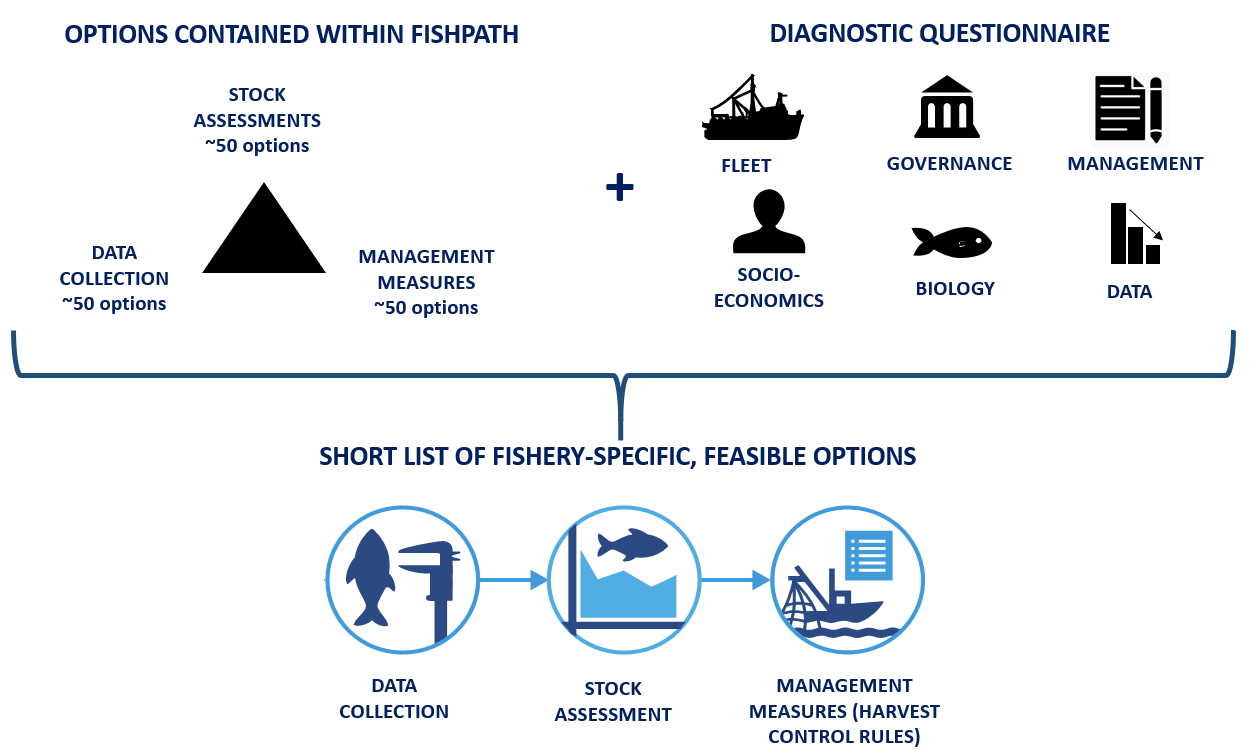
\includegraphics[width=0.75\linewidth]{images/fishpath-tool-overview-diagram} 

}

\caption{The FishPath tool at a glance.}\label{fig:overview}
\end{figure}

\hypertarget{purpose-and-intended-audience-of-the-fishpath-tool-user-guide}{%
\section{Purpose and Intended Audience of the FishPath Tool User Guide}\label{purpose-and-intended-audience-of-the-fishpath-tool-user-guide}}

The purpose of the FishPath Tool User Guide is to orient users to the FishPath tool, explain the functionality of tool features, and provide succinct guidance on how to use the FishPath tool to select and review appropriate harvest strategy options. The ultimate goal of using the FishPath Tool is to support the development of an articulated harvest strategy for use in a Fishery Management Plan (this process is outside the scope of the FishPath Tool User Guide).

The FishPath tool is applicable in a variety of settings. Examples include: use of the FishPath tool in a facilitated, multi-stakeholder workshop setting; small expert groups; individual (``desktop'') use for harvest strategy development or review; or research related to individual components of a harvest strategy, such as selection of an assessment method or details about specific data collection or management measure options. The impact of the tool greatly depends on the context it is used, being most effective in a multi-stakeholder process and lead by experienced practitioners. The use of the tool can also be adapted to work with multi-species fisheries, multi-fleet fisheries, and in selecting current and future scenarios. Guidance on using the tool in these contexts will be incorporated into future versions of the user guide.

\hypertarget{starting-the-fishpath-tool}{%
\chapter{Starting the FishPath Tool}\label{starting-the-fishpath-tool}}

Importantly, the FishPath tool requires a consistent internet connection to access the questionnaire, save answers, and interact with results.

\hypertarget{welcome-page}{%
\section{Welcome Page}\label{welcome-page}}

When a user navigates to \url{https://tool.fishpath.org/}, a welcome page is displayed with two prompts: ``Create an Account'' or ``Login'' (Figure \ref{fig:welcome}).

\begin{figure}

{\centering 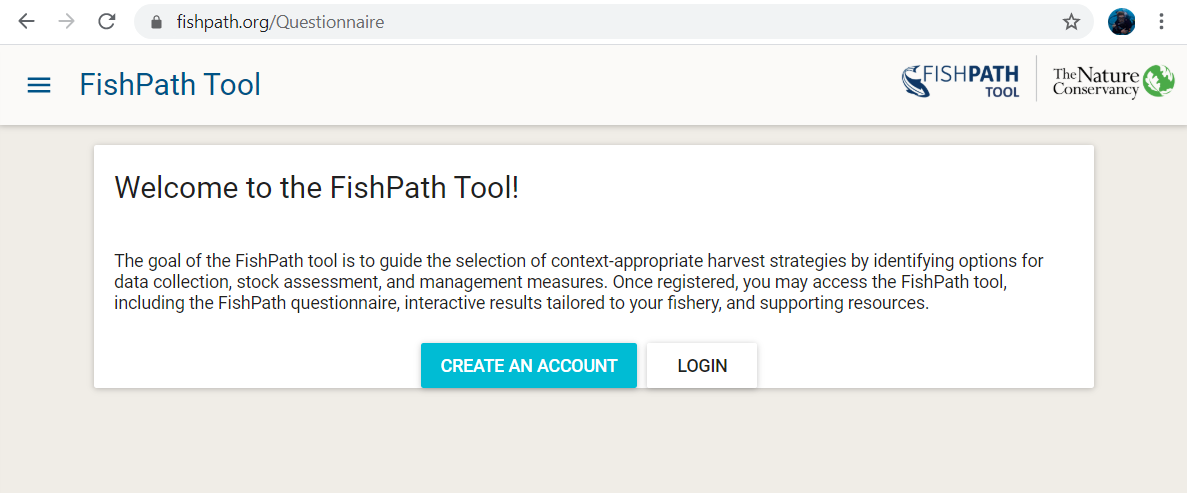
\includegraphics[width=0.95\linewidth]{images/welcome-page} 

}

\caption{Welcome page of the FishPath tool.}\label{fig:welcome}
\end{figure}

\hypertarget{creating-a-fishpath-account}{%
\section{Creating a FishPath Account}\label{creating-a-fishpath-account}}

Upon selecting ``Create an Account'', a pop-up window appears with the following fill-in fields (Figure \ref{fig:create-account}). An asterisk denotes mandatory information.

\begin{itemize}
\tightlist
\item
  Email*
\item
  Password* (create a password)
\item
  Organization Type*
\item
  Organization
\item
  Your Name*
\item
  Country*
\end{itemize}

Note that the email and password fields are case sensitive.

This information is used to track user origin and the use of the FishPath tool. At this account creation stage, the user is also prompted to read and accept the Terms of Service of the FishPath tool, developed by The Nature Conservancy (\protect\hyperlink{terms}{Appendix B}).

\begin{figure}

{\centering 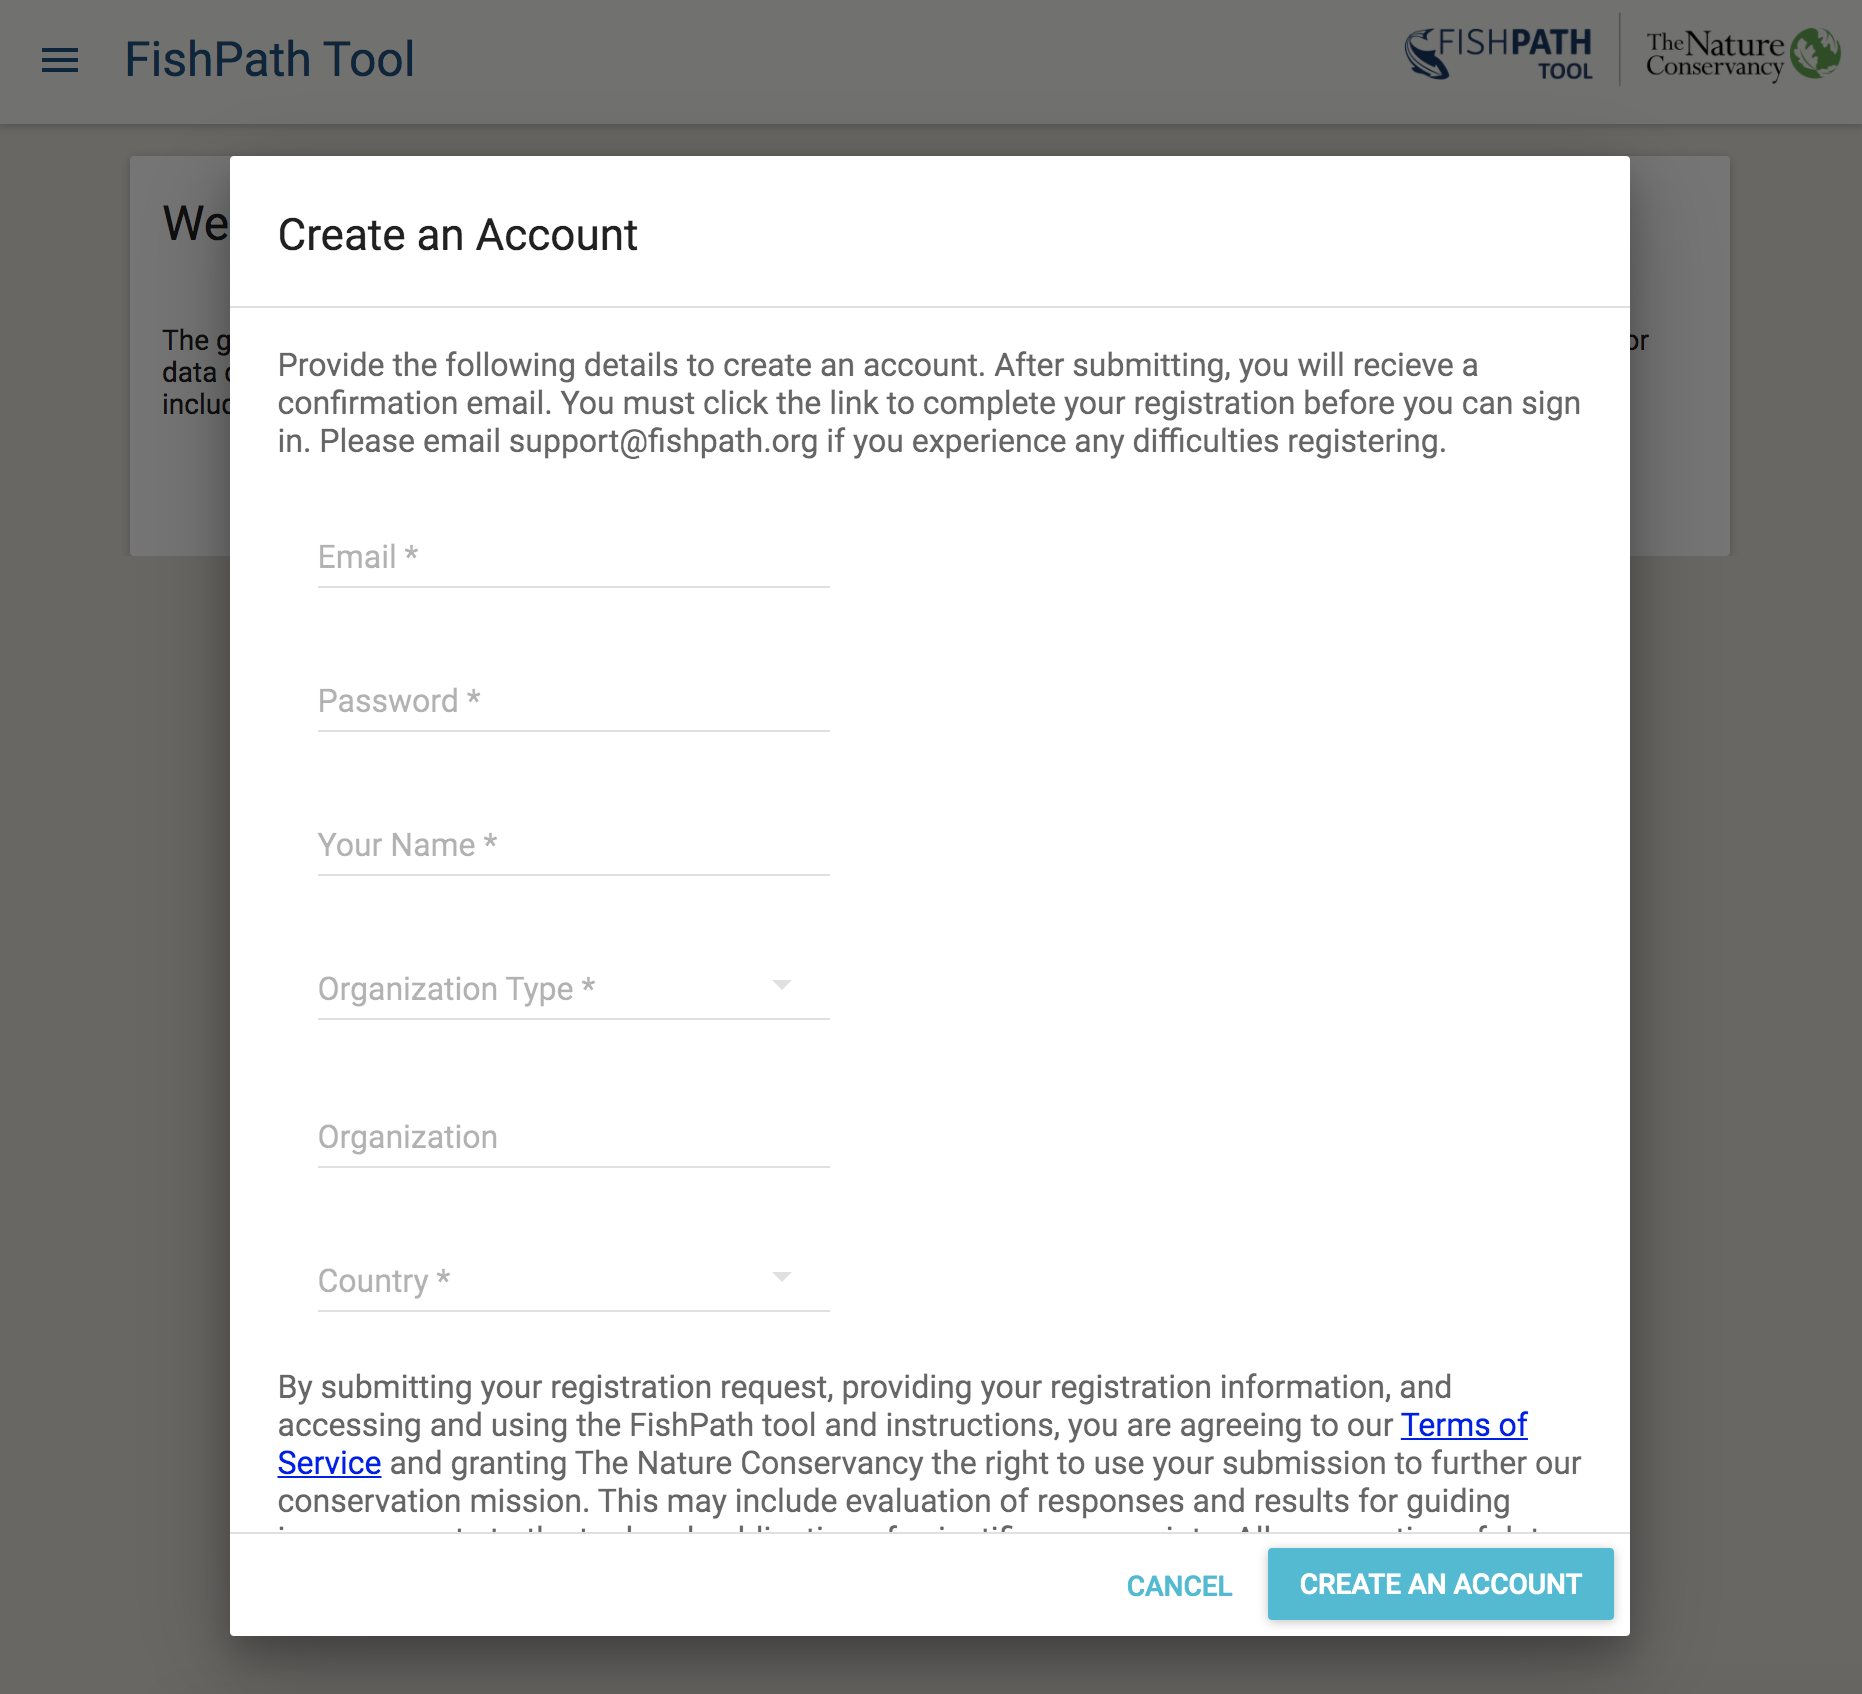
\includegraphics[width=0.95\linewidth]{images/create-account} 

}

\caption{“Create an Account” screen of the FishPath tool.}\label{fig:create-account}
\end{figure}

After submitting the account request, the user will receive a confirmation email with a link to complete registration. After account creation, whenever the user returns to the Welcome Page of the FishPath tool, the user may simply ``Login'' with their email address and password (Figure \ref{fig:login-page}).

\begin{figure}

{\centering 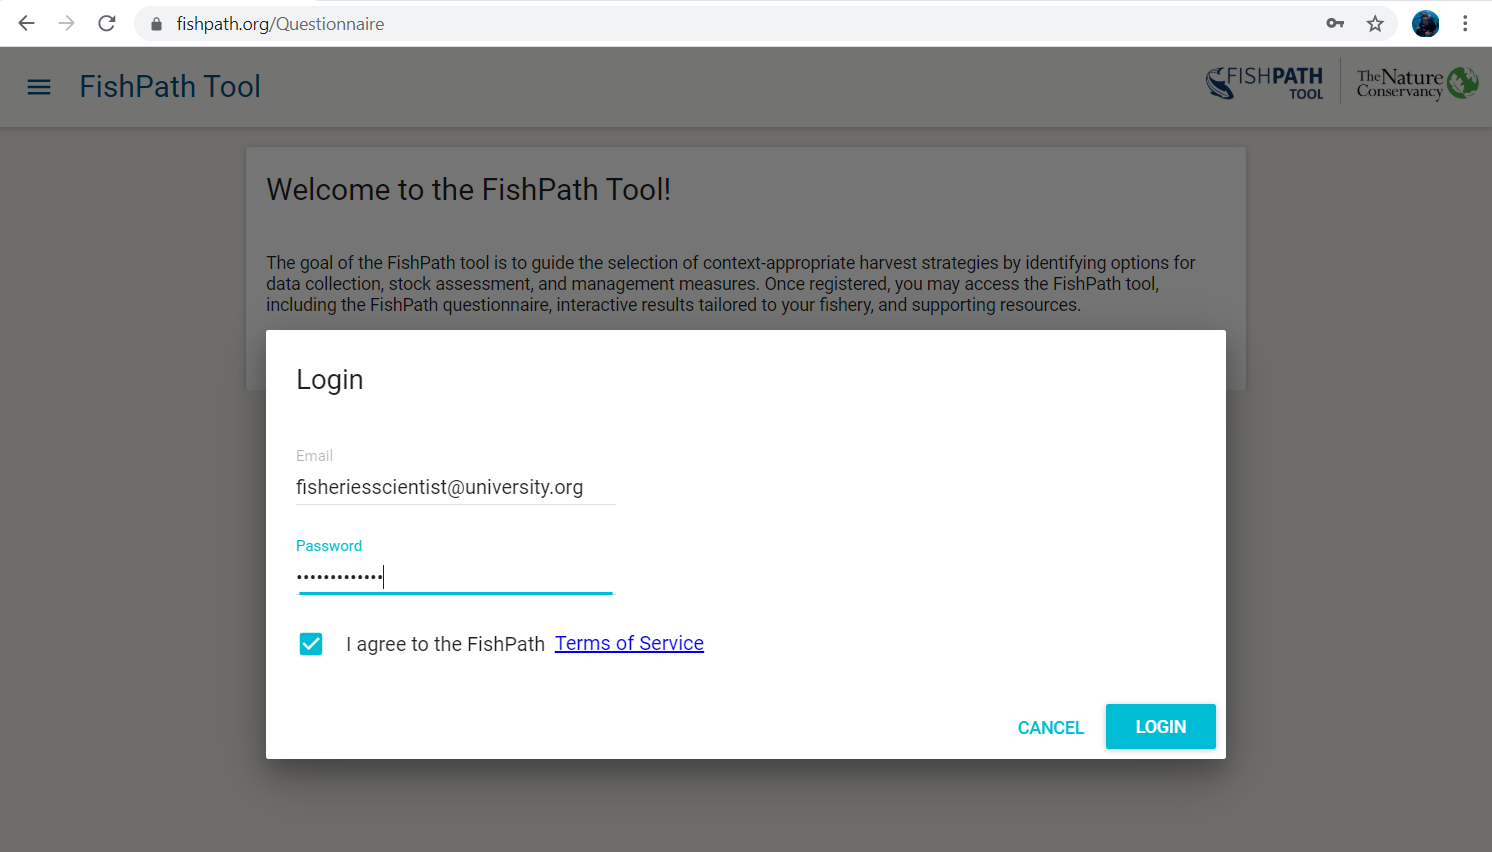
\includegraphics[width=0.95\linewidth]{images/login-page} 

}

\caption{Login Page of the FishPath tool.}\label{fig:login-page}
\end{figure}

\hypertarget{fishpath-tool-dashboard}{%
\section{FishPath Tool Dashboard}\label{fishpath-tool-dashboard}}

After creating an account (new user) or logging in (existing user), the user is directed to the FishPath Tool Dashboard (Figure \ref{fig:dashboard}), or the user's ``homepage'' of the FishPath Tool. On the FishPath Tool Dashboard, users view 4 headings:

\begin{enumerate}
\def\labelenumi{\arabic{enumi}.}
\tightlist
\item
  \textbf{``FishPath Tool User Guide''}, which contains detail on using the FishPath Tool and interpreting results.
\item
  \textbf{``My Fisheries''}, which provides a list of the user's current list of fisheries they have started or completed in the tool. Users may access their fisheries at any time through this section, and return to in-progress FishPath questionnaires or results pages;
\item
  \textbf{``Reference Materials''}, which provides a list of all options contained in the FishPath tool with details and reference materials;
\item
  \textbf{``Help us improve the FishPath Tool''}, which allows the user to send feedback to the FishPath team.
\end{enumerate}

\begin{figure}

{\centering 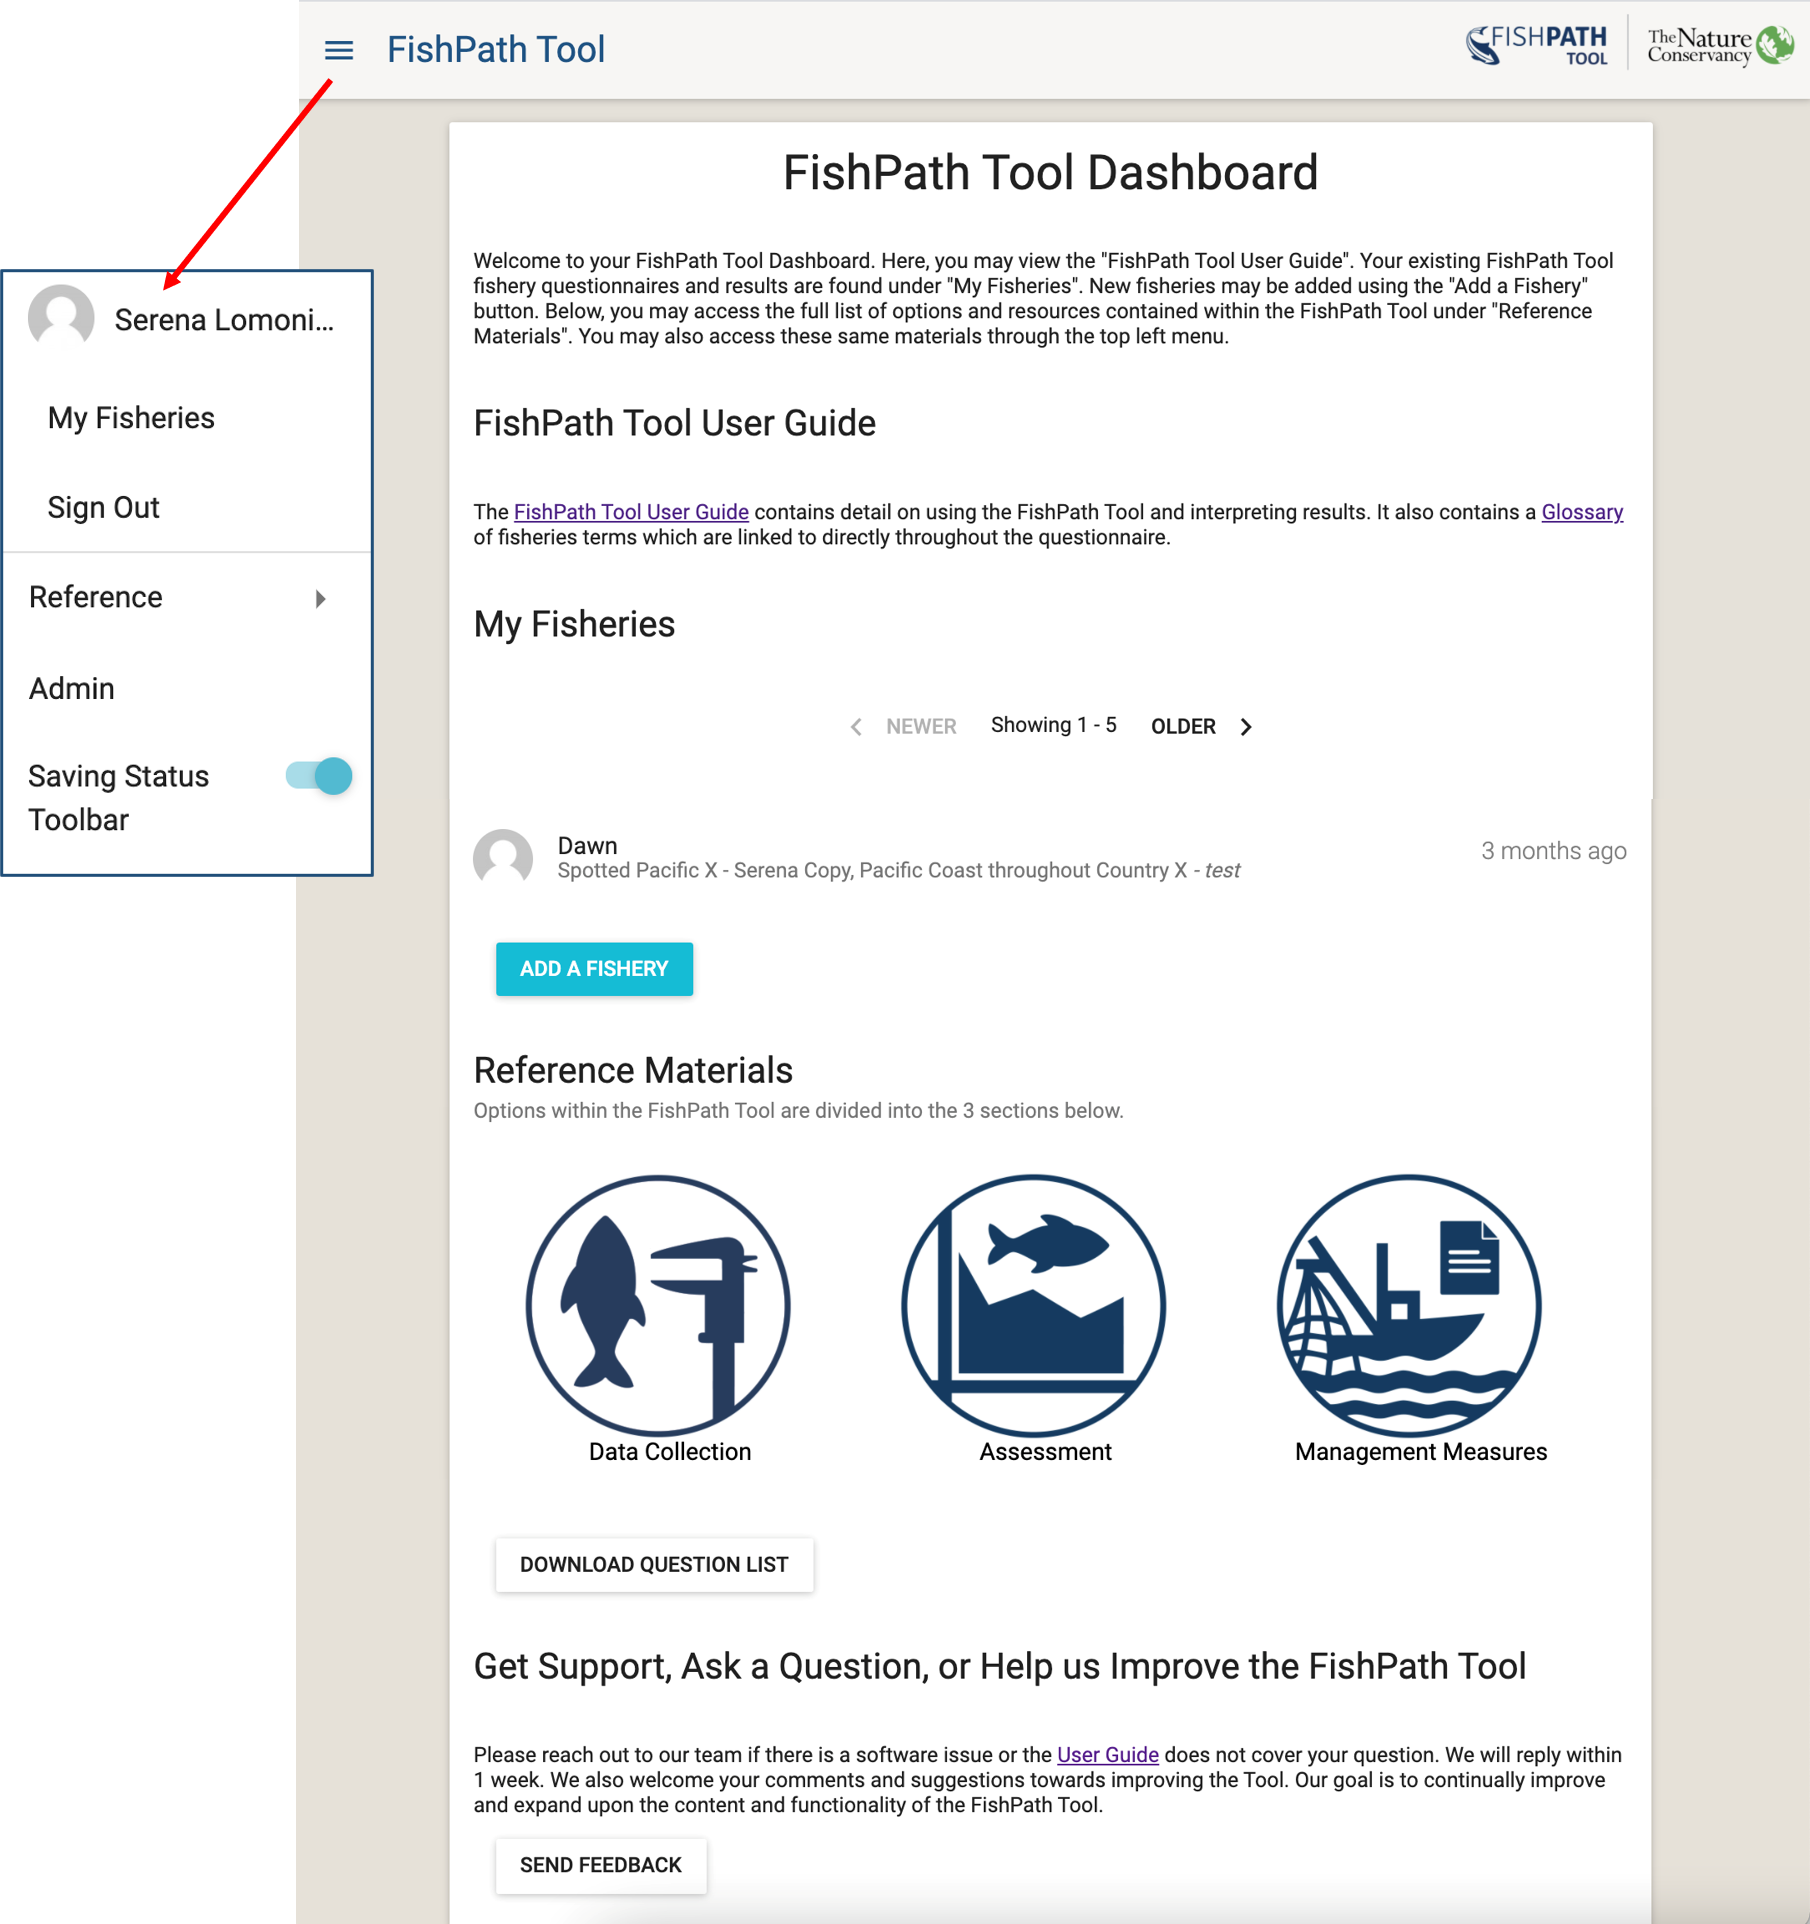
\includegraphics[width=0.95\linewidth]{images/user-dashboard} 

}

\caption{FishPath Tool Dashboard, or the homepage for FishPath tool users. The pop out shows the FishPath Tool Dashboard drop-down menu.}\label{fig:dashboard}
\end{figure}

When a user clicks the ``FishPath Tool'' menu in the top left corner, a drop-down display allows the user to navigate to various options (Figure \ref{fig:dashboard}). The ``Reference Materials'' tab displays all of the options contained in the FishPath Tool.

\hypertarget{adding-a-new-fishery}{%
\section{Adding a New Fishery}\label{adding-a-new-fishery}}

Selecting the blue button ``Add a Fishery'' allows users to start a new fishery in the FishPath tool that will be added to their account. First, a pop-up ``Fishery Information'' screen appears to prompt users to define the fishery of focus (Figure \ref{fig:fishery-info}), using the fields below. This information is used to better understand the use of the FishPath tool, provide high-level aggregate information about fishery characteristics, and to help users define the fishery to which they will be applying FishPath, so that answers will be directed at that fishery only.

\begin{itemize}
\tightlist
\item
  Fishery Common Name(s):
\item
  Genus species:
\item
  Fleet and Gear Type(s):
\item
  Country or Countries:
\item
  Geographic Area of the Fishery:
\item
  In which of these 3 contexts is the FishPath Tool being used for this fishery?

  \begin{itemize}
  \tightlist
  \item
    Exploratory test run\\
  \item
    Facilitated workshop for specific fishery
  \item
    Individual use for specific fishery
  \end{itemize}
\end{itemize}

\begin{figure}

{\centering 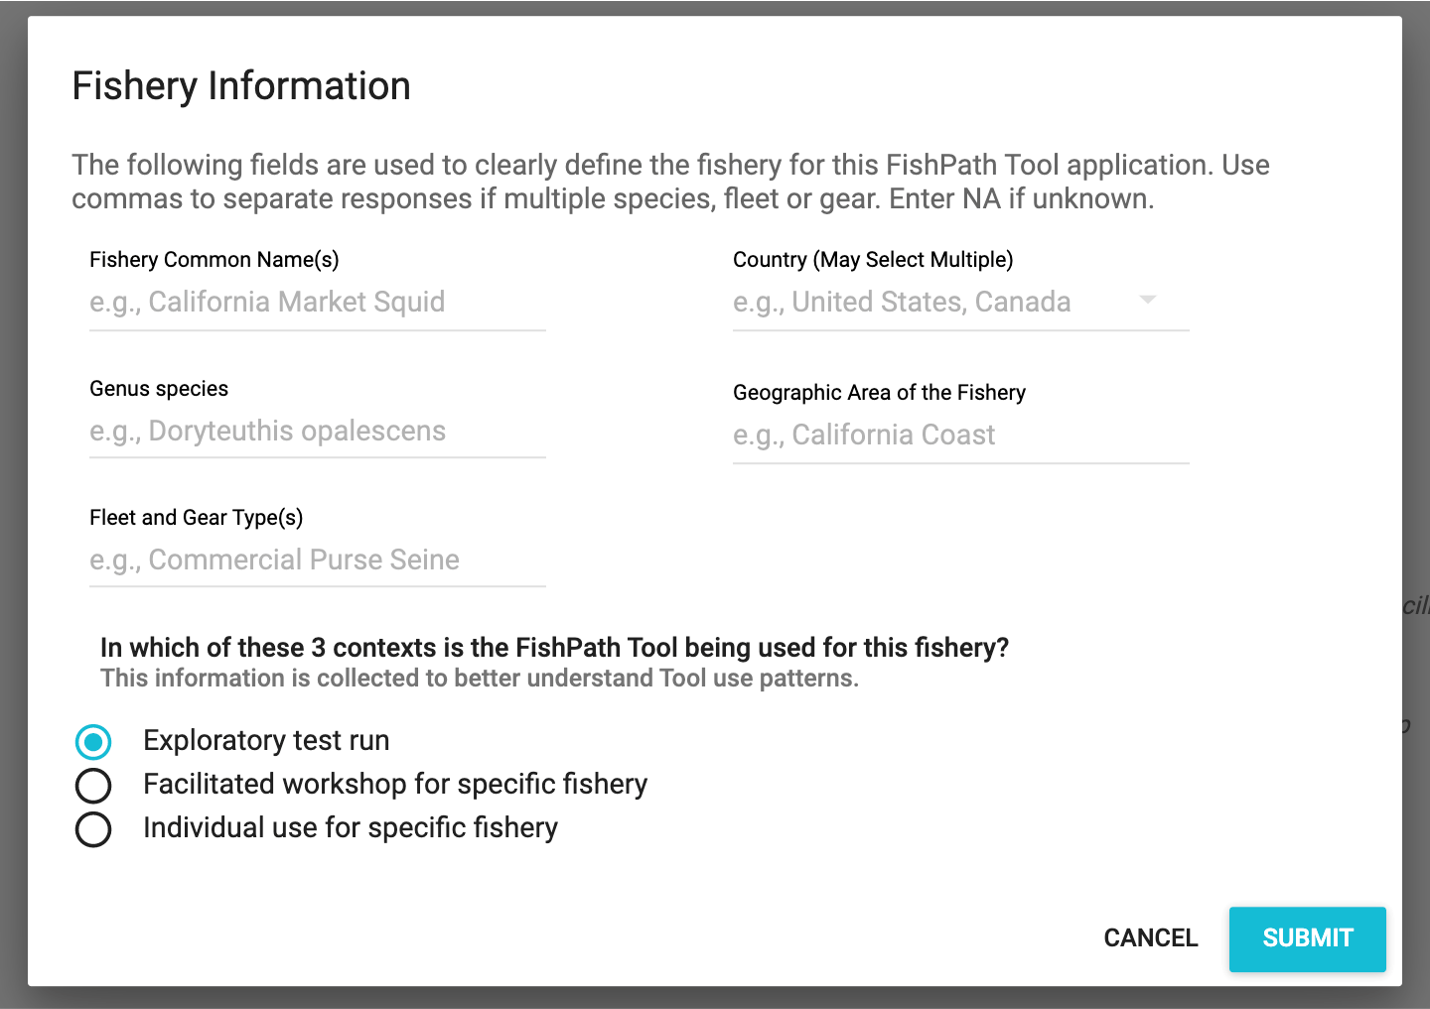
\includegraphics[width=0.95\linewidth]{images/fishery-info-screen} 

}

\caption{Fishery Information pop-up screen of the FishPath Tool.}\label{fig:fishery-info}
\end{figure}

Upon selecting ``Submit'', the user is prompted to select one of the 3 harvest strategy components (sections) of the FishPath Tool (Data Collection, Assessment, Management Measures) and begin the FishPath tool questionnaire (Figure \ref{fig:fishery-entry}). Users can complete and review results from these sections independently. A pencil in the upper-right corner allows users to edit the fishery information (input in Figure \ref{fig:fishery-entry}) at any time.

\begin{figure}

{\centering 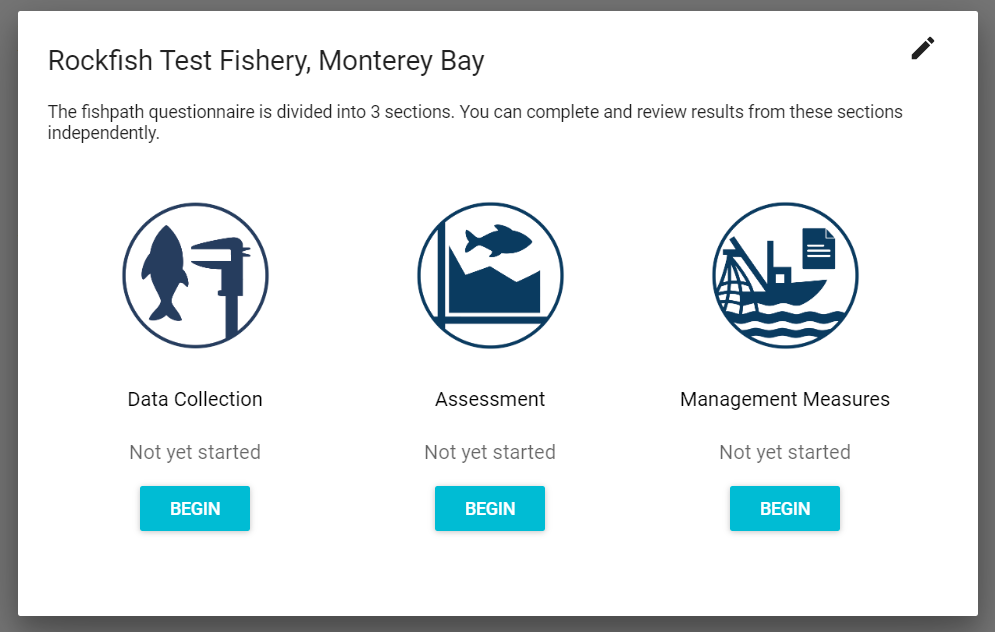
\includegraphics[width=0.95\linewidth]{images/fishery-entry-screen} 

}

\caption{Entry screen to the FishPath tool questionnaire after fishery information has been defined.}\label{fig:fishery-entry}
\end{figure}

\hypertarget{fishpath-tool-questionnaire}{%
\chapter{FishPath Tool Questionnaire}\label{fishpath-tool-questionnaire}}

The goal of the FishPath tool questionnaire is to elicit information about all aspects of the fishery. This information leads to the activation of assumptions, cautions and considerations for each option. Across the three sections (Data Collection, Assessment, and Management Measures) the user answers a series of \textasciitilde120 questions. Questions are categorized in 6 categories, which indicate the nature of the information in the question:

\begin{enumerate}
\def\labelenumi{\arabic{enumi}.}
\tightlist
\item
  Biology/Life History
\item
  Data Availability
\item
  Governance
\item
  Management
\item
  Operational Characteristics
\item
  Socio-Economic
\end{enumerate}

Some questions span multiple sections of the questionnaire (i.e.~they are relevant in considering multiple components of a harvest strategy). To avoid duplicity, such questions, once answered, will show as completed when beginning any subsequent section in which they occur.

At any time, the user may close and later return to their session via their ``My Fisheries'' dashboard. Any submitted answers will be saved with a consistent internet connection. Once the user has completed an individual section, which may only be achieved by providing responses to all questions in that section, the user may either complete a subsequent section or view results from the completed section. Results for any section become available once the user has completed the respective questionnaire. The questionnaire is periodically updated by the FishPath team to reflect the latest fisheries science, so users may need to answer any new questions when returning to a fishery before reviewing results of associated sections.

After viewing the entry screen to the FishPath questionnaire (Figure \ref{fig:fishery-entry}), the user selects one of the 3 sections. An overview screen will appear with the name of the section, the number of questions associated with that section, and a short guidance on answering the questions (Figure \ref{fig:dc-overview}). The user can then choose to ``Begin'' the section or ``Choose Another Section''.

\begin{figure}

{\centering 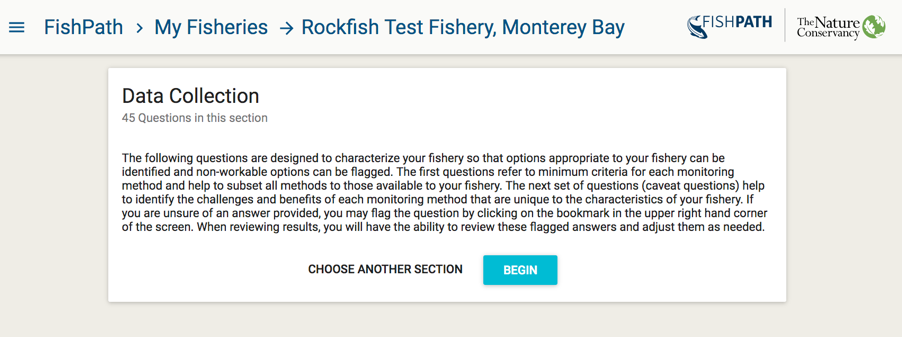
\includegraphics[width=0.95\linewidth]{images/dc-overview} 

}

\caption{Data Collection section overview.}\label{fig:dc-overview}
\end{figure}

\hypertarget{criteria-and-caveat-questions}{%
\section{Criteria and Caveat Questions}\label{criteria-and-caveat-questions}}

In the FishPath tool, questions are designated as either ``Criteria'' or ``Caveats'' or both, which refers to how question responses are linked to options contained within FishPath.

A Criterion question is used to determine whether the fishery meets a minimum qualification required to apply an option. Whether the fishery meets the minimum (or often multiple) criteria for each option is indicated in the results window (see Results sections below). For example, in the ``Assessment'' section of the questionnaire, there are questions about data quality, quantity, and data type for the fishery, which correspond to the minimum levels required to enable each type of assessment method. Upon answering a ``criteria question'' about, for example, fishing effort data, within the Assessment section (Figure \ref{fig:ex-crit-question}), the fishery will be scored in the results section according to whether it meets that particular minimum level of effort data required by particular assessment options. The Results section reports not only whether or not each criterion is met, but also gives an indication, via subjectively assigned traffic light color scales, as to the degree the criteria is met, and provides guidance as to the level of uncertainty associated with that particular required input. Criteria questions are not included in the ``Management Measures'' section. While a management measure option may be ill-advised because it violates assumptions (i.e, ``caveats''), there are no prohibiting factors that would prevent any single option being implemented, if so desired. Conversely, one cannot undertake certain assessments or forms of data collection without meeting minimum requirements.

Questions whose responses invoke ``caveats'' will not eliminate or retain options, but rather invoke subjectively assigned traffic light-colored warnings, or positive attributes, against specific options. These are intended to speak to issues that do not necessarily prohibit the option's feasibility, but that should be given explicit consideration, and the ability to address each should be determined, before deeming the option is best suited to the fishery. As with the criteria questions, these are presented in the results section of the FishPath tool with explanatory text.

\begin{figure}
 
 {\centering 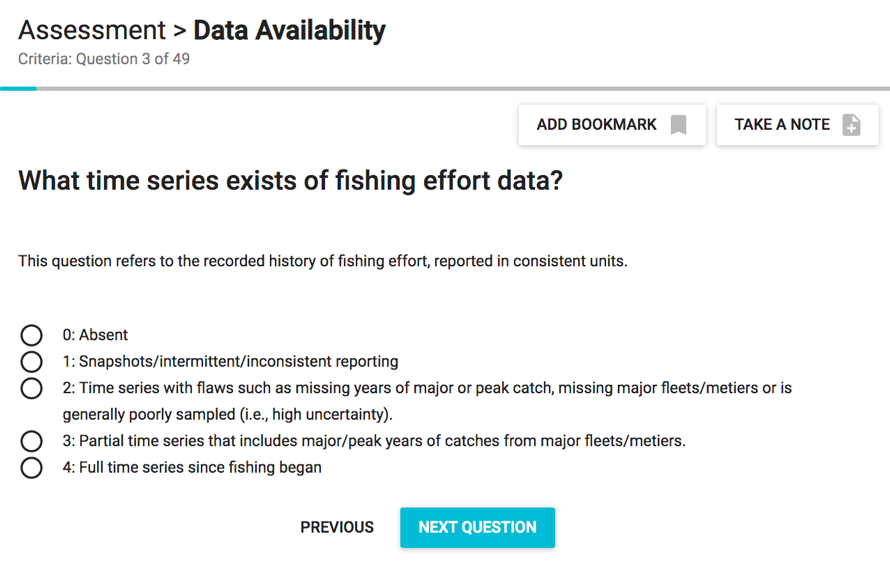
\includegraphics[width=0.95\linewidth]{images/ex-crit-question} 
 
 }
 
 \caption{Example “criteria” question in the Assessment section of the FishPath Questionnaire.}\label{fig:ex-crit-question}
 \end{figure}

\hypertarget{anatomy-of-a-fishpath-tool-question}{%
\section{Anatomy of a FishPath Tool Question}\label{anatomy-of-a-fishpath-tool-question}}

(Figure \ref{fig:question-anatomy}) provides an example of a FishPath question screen:

\begin{enumerate}
\def\labelenumi{\arabic{enumi}.}
\tightlist
\item
  At the top of the screen, the \textbf{section} is shown (either Data Collection, Assessments, or Management Measures).
\item
  The section is followed by the \textbf{question category} (i.e., Biology/Life History, Data Availability, Governance, Management, Operational Characteristics, or Socio-Economic).
\item
  A sub-heading identifies whether the question is a \textbf{``criteria'' or a ``caveat''} question.
\item
  The sub-heading also indicates the \textbf{number of questions answered} and remaining within that section.
\item
  For the Data Collection section only, it is also stated whether the question pertains to either issues of \textbf{``representation'' or ``implementation''}. This helps users to understand the intent of the question, by identifying whether the question has ramifications for the form of data collection in terms of its either ability to obtain representative data, or in its ability to be effectively implemented.
\item
  There is the ability to \textbf{``Bookmark''} the question. A bookmark flags questions for ease of later revisiting (Figure \ref{fig:bookmark-notes}). A question may be bookmarked for reasons such as if the answer is unknown, it needs further consideration or input, is in dispute, or if the user feels the question is critical. As all questions must be answered in order to review results, adding a bookmark allows users to provide an interim response that may be revisited in the results section, once the user can evaluate the relative impact of their response.
\item
  Users can \textbf{``Take A Note''} on a question (Figure \ref{fig:bookmark-notes}). Notes can be taken for a variety of reasons such as to clarify why a certain response was given, to capture important discussion had about a question, why the question was bookmarked or noting a response requiring further research. Notes can later form an important part of draft harvest strategy development, and, by providing justification for the response, can maintain traceability and replicability. When connected to the internet, all notes made will be saved into FishPath and available to the user for reference.
\item
  At the bottom of the screen, the user may advance to the \textbf{next question} or return to the \textbf{previous} question.
\end{enumerate}

\begin{figure}
 
 {\centering 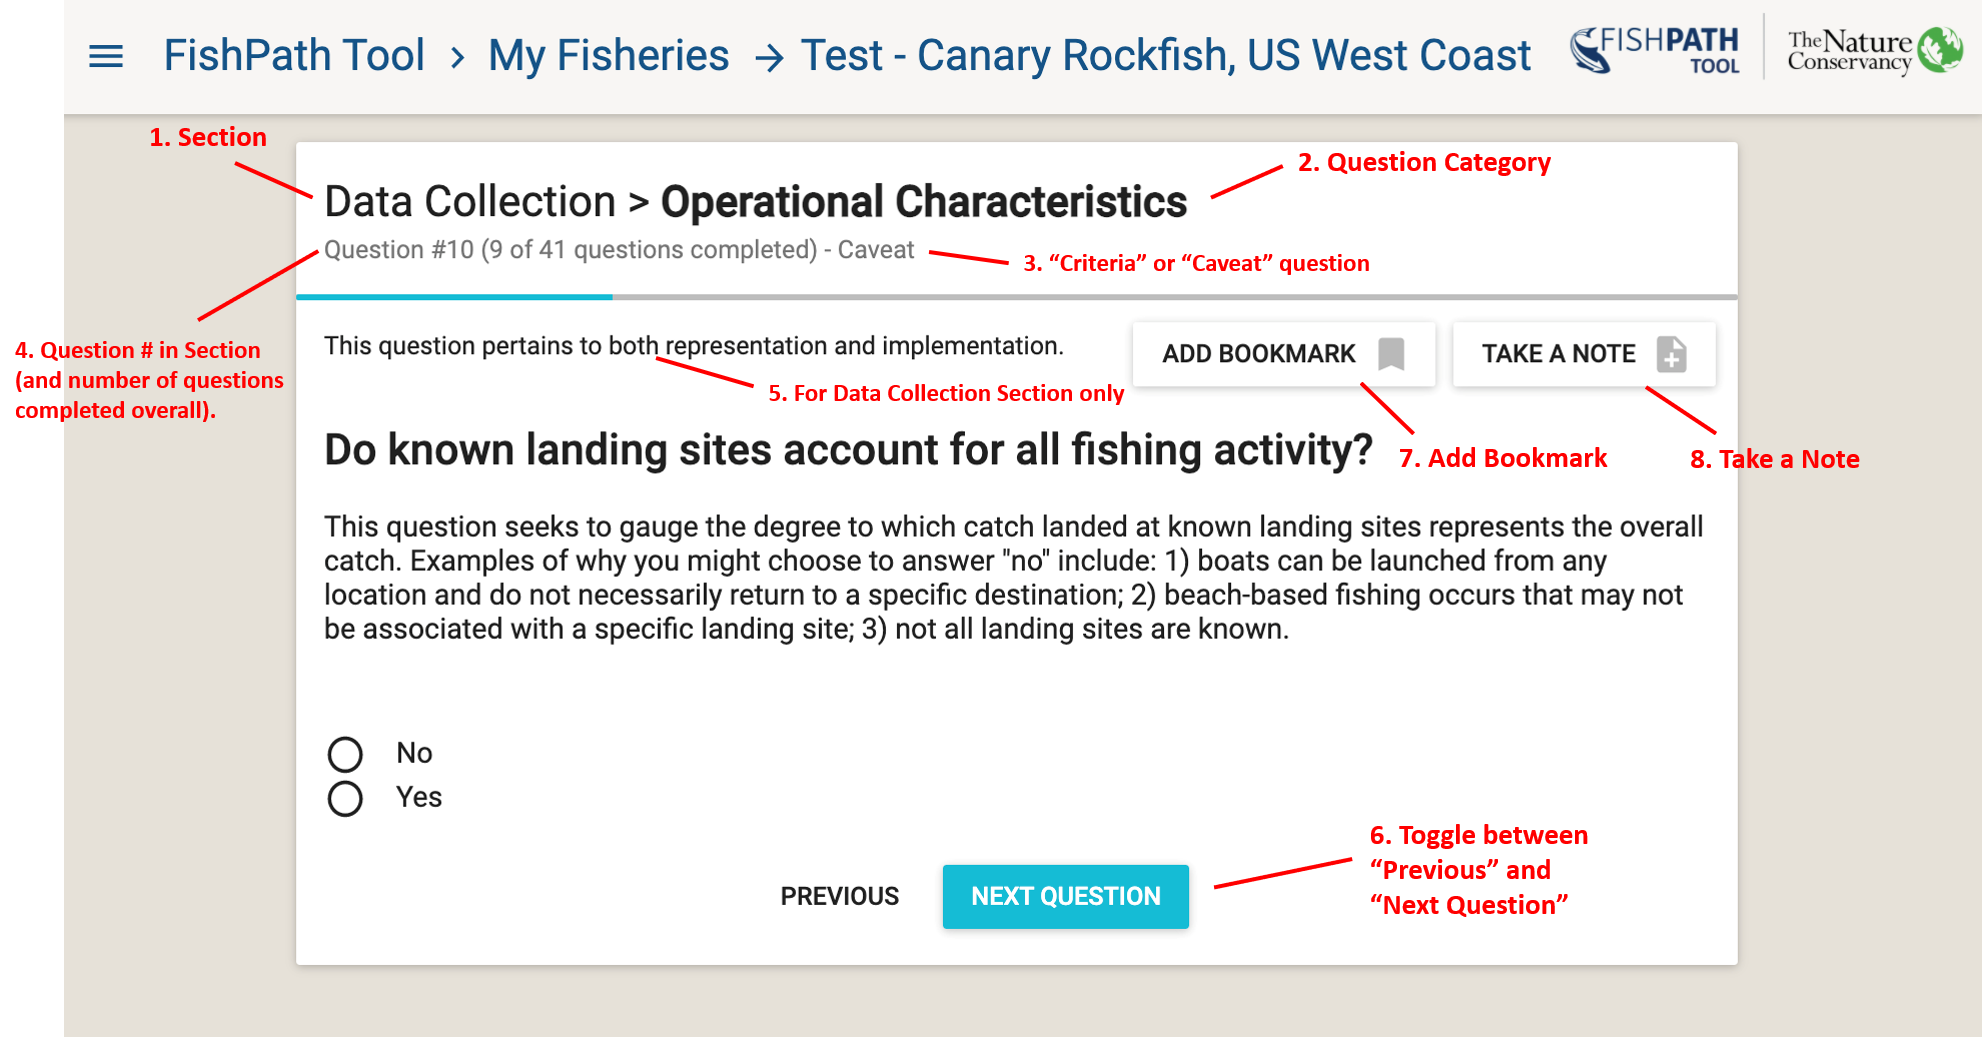
\includegraphics[width=0.95\linewidth]{images/question-anatomy} 
 
 }
 
 \caption{Anatomy of a FishPath tool question.}\label{fig:question-anatomy}
 \end{figure}

\begin{figure}
 
 {\centering 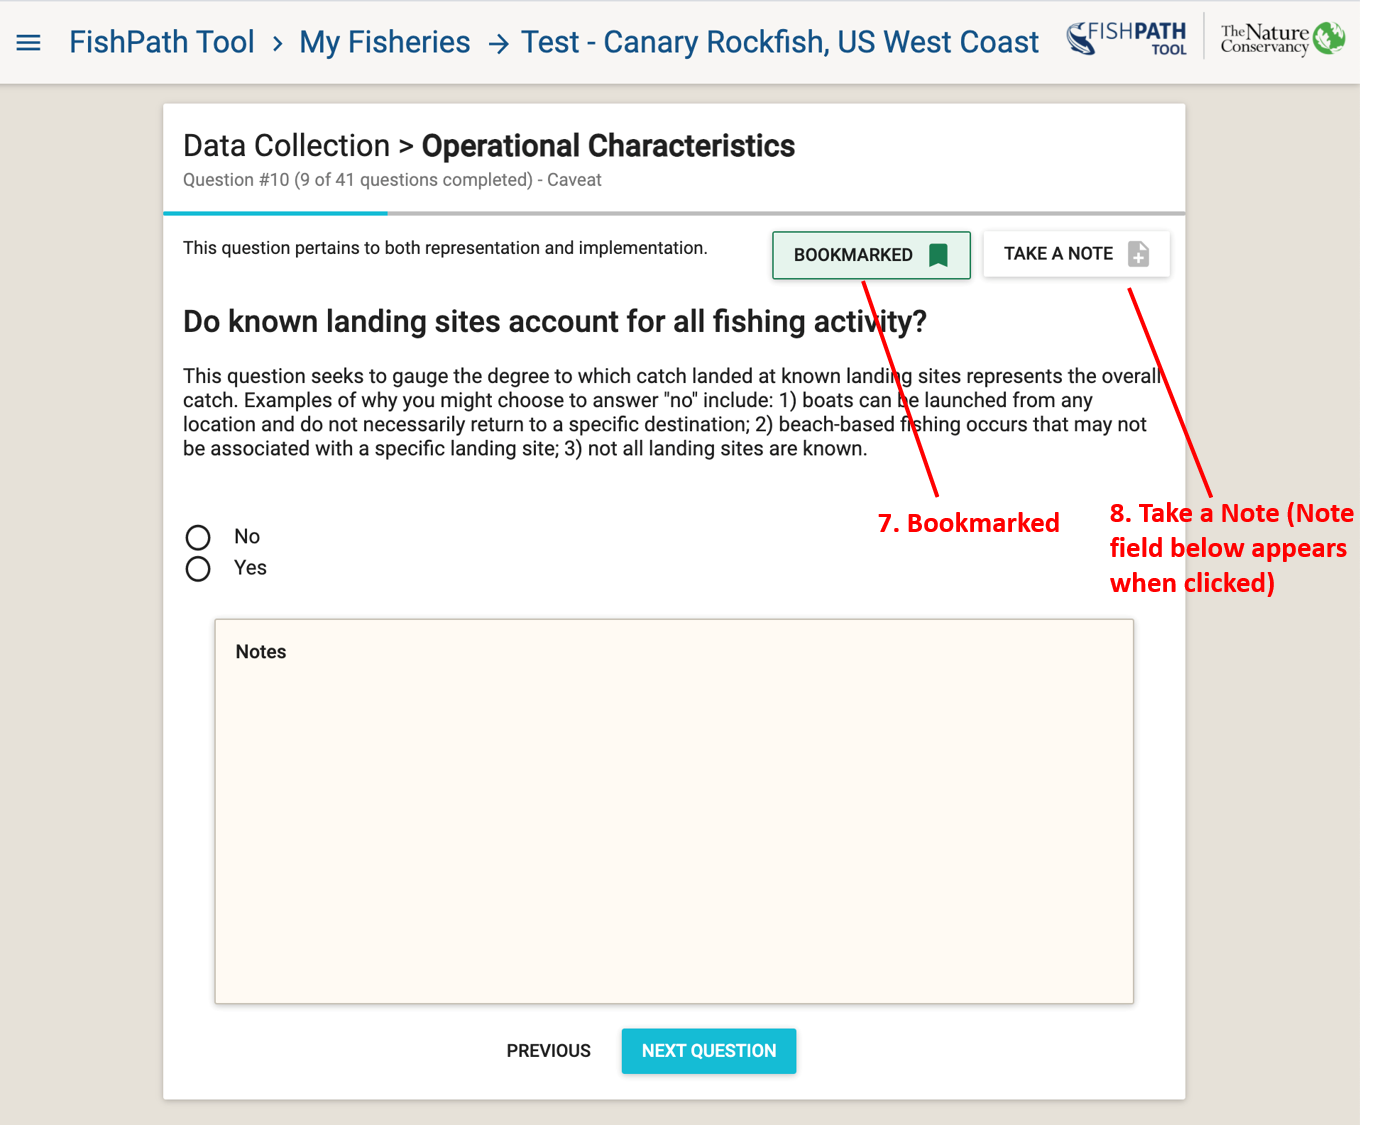
\includegraphics[width=0.95\linewidth]{images/bookmark-notes} 
 
 }
 
 \caption{Example FishPath tool question with “Bookmark” (green) and “Take a note” (text box) functionality selected.}\label{fig:bookmark-notes}
 \end{figure}

\hypertarget{subjective-questions}{%
\section{Subjective Questions}\label{subjective-questions}}

While the majority of questions within FishPath are intended to be answered definitively (objective), certain questions are subjective in nature. The latter typically request a user response in the form of a perceived ranking (e.g.~``low'', ``moderate'', ``high''). Most such questions invoke caveats and, when all caveats are considered together, the relative impact of those invoked by subjective questions can be evaluated. In this way, priority can be assigned to whether the response requires further consideration and debate, or whether it is of little relative significance in determining the most viable harvest strategy options. Further discussion can then be focused on the most appropriate issues.

Generally, the best approach to take when completing the questionnaire is to aim to do so relatively efficiently, without overtly laboring or debating over any one question. If in doubt, the question can be bookmarked, and notes can be taken, for easy revisiting later. The transparency of the FishPath tool is such that users will be able to see explicitly how their response to any one question influences the results (by invoking criteria or caveats), and to readily change their answer if so desired. Moreover, the aim of the questionnaire is to obtain an overall profile of the fishery's characteristics, so as best to inform the choice of harvest strategy option. As such, questions may pertain to only a few options, or they may not invoke strong caveats. The goal is to appraise the fishery as a whole, as opposed to focusing on any single question.

\hypertarget{completing-the-questionnaire}{%
\section{Completing the Questionnaire}\label{completing-the-questionnaire}}

Upon completing or exiting any of the three sections, a summary screen appears with the status of relative completion. Users review their result for completed sections, or otherwise continue the questionnaire (Figure \ref{fig:summary-screen}).

\begin{figure}
 
 {\centering 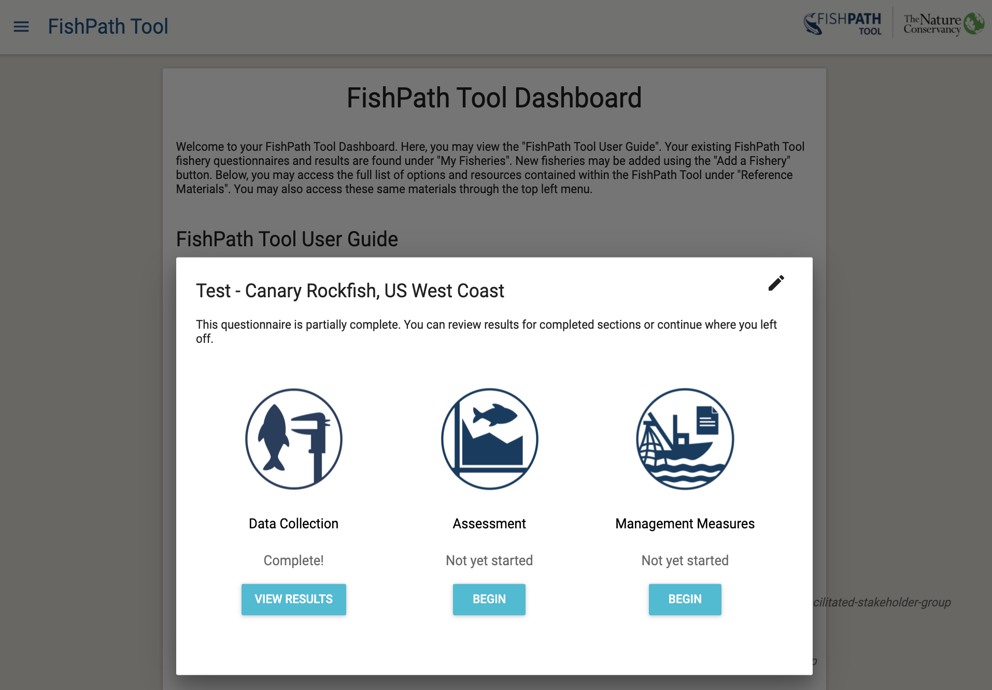
\includegraphics[width=0.95\linewidth]{images/summary-screen} 
 
 }
 
 \caption{Summary window of the 3 FishPath questionnaire sections, showing questionnaire progress.}\label{fig:summary-screen}
 \end{figure}

\hypertarget{fishpath-tool-interactive-results-page}{%
\chapter{FishPath Tool Interactive Results Page}\label{fishpath-tool-interactive-results-page}}

The FishPath Tool Interactive Results Pages allow users to view and interact with all of the options contained within FishPath and understand how each option may apply to their fishery.

Upon completion of the questionnaire for any section, the user is directed to the FishPath Tool Interactive Results page (Figure \ref{fig:results-overview}). The results are presented separately for each of the 3 sections, or harvest strategy component: 1) Data Collection; 2) Assessment; and 3) Management Measures (Figure \ref{fig:results-overview}, sections shown in dark blue bars near top of screen).

Each of the three sections of the results can be accessed individually without needing to complete all three sections. If a user has not completed the questionnaire in at least one of the sections, they will be prompted to return to finish the section questionnaire before accessing results (Figure \ref{fig:summary-screen}).

\begin{figure}

{\centering 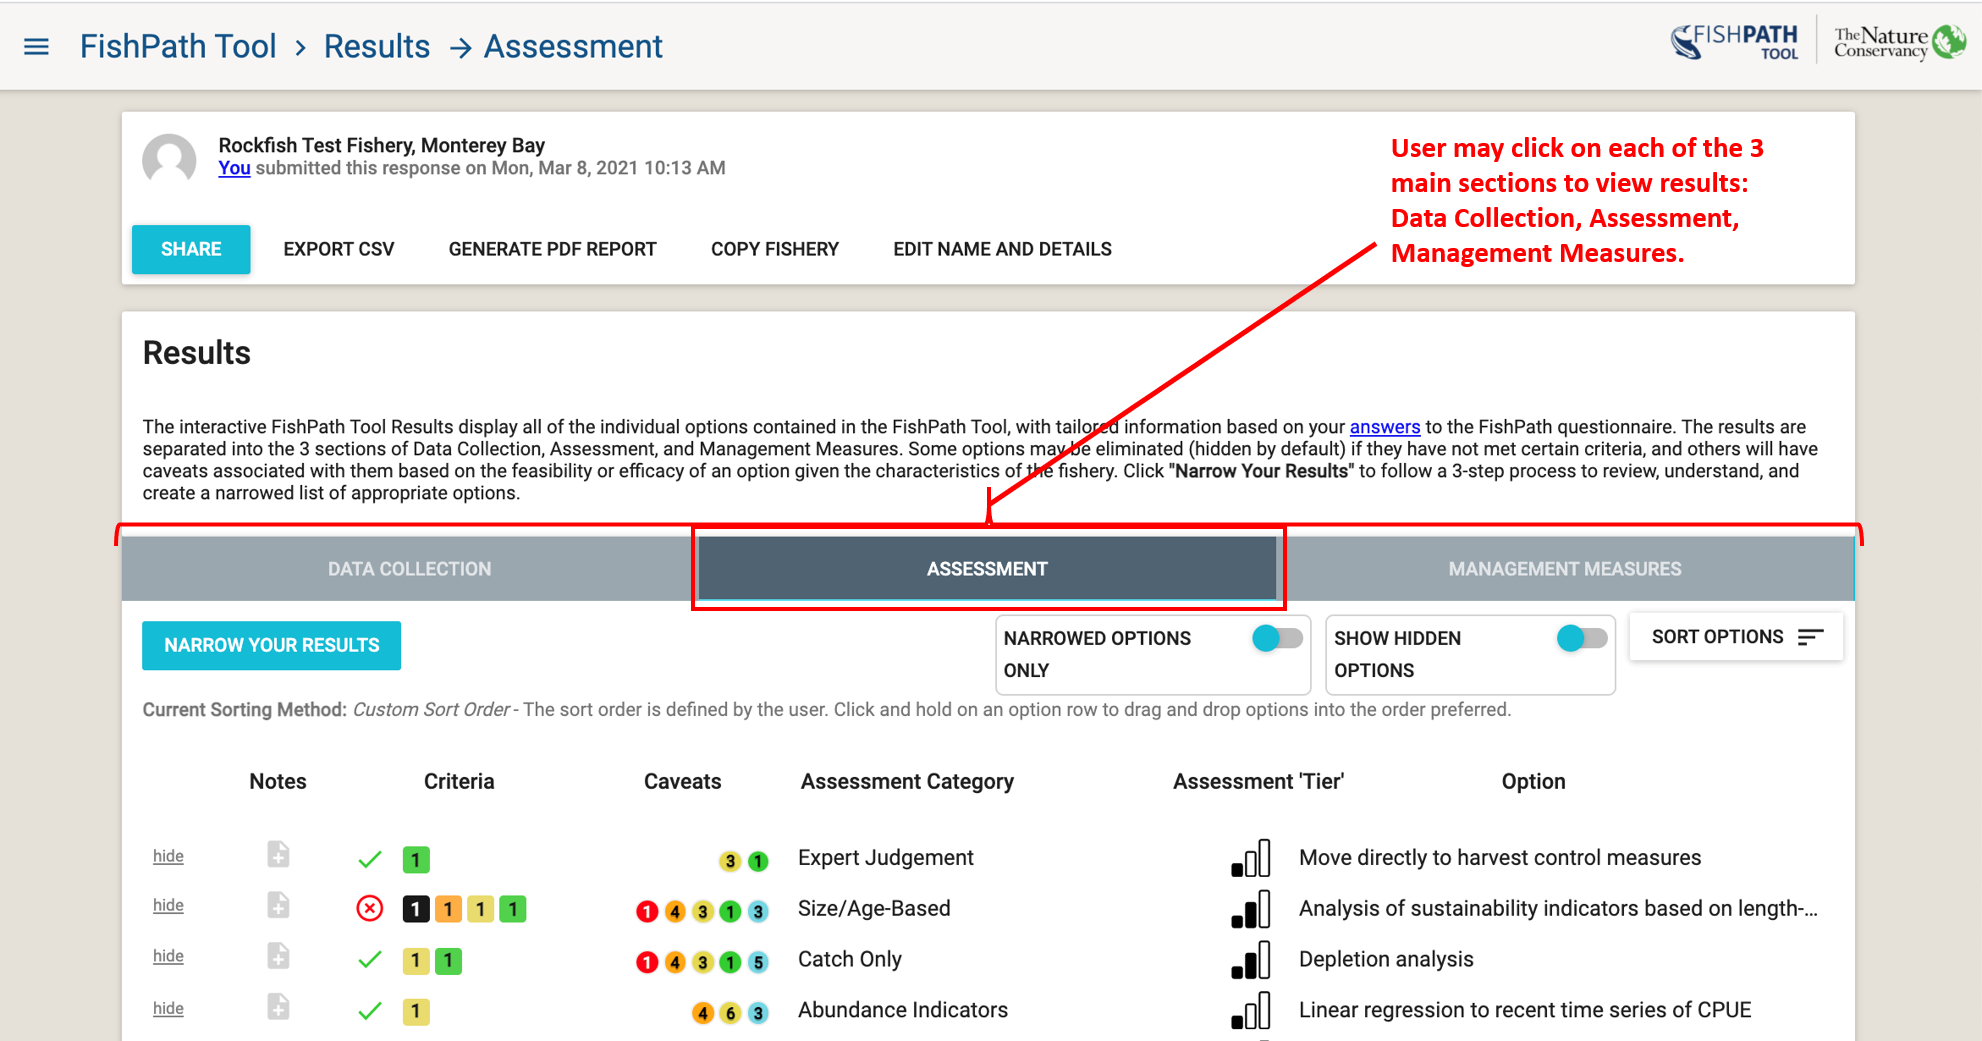
\includegraphics[width=0.95\linewidth]{images/results-overview} 

}

\caption{Initial results display screen in the FishPath tool (featuring the Assessment section), displaying a snapshot of results, not a full listing.}\label{fig:results-overview}
\end{figure}

Figure \ref{fig:results-components} shows the general components of the results page. Each of these is elaborated below:

\begin{enumerate}
\def\labelenumi{\arabic{enumi}.}
\tightlist
\item
  \protect\hyperlink{Results-Actions}{Actions to Share Results and Edit Fishery Info}
\item
  \protect\hyperlink{interactive-results-table}{Interactive Results Table}
\item
  \protect\hyperlink{show-hidden-options-and-sort-options}{Show Hidden Options and Sort Options}
\item
  \protect\hyperlink{bookmarked-questions-and-influential-answers}{Bookmarked Questions and Influential Answers}
\item
  \protect\hyperlink{Results-Narrowing}{Results Narrowing Process}
\end{enumerate}

\begin{figure}

{\centering 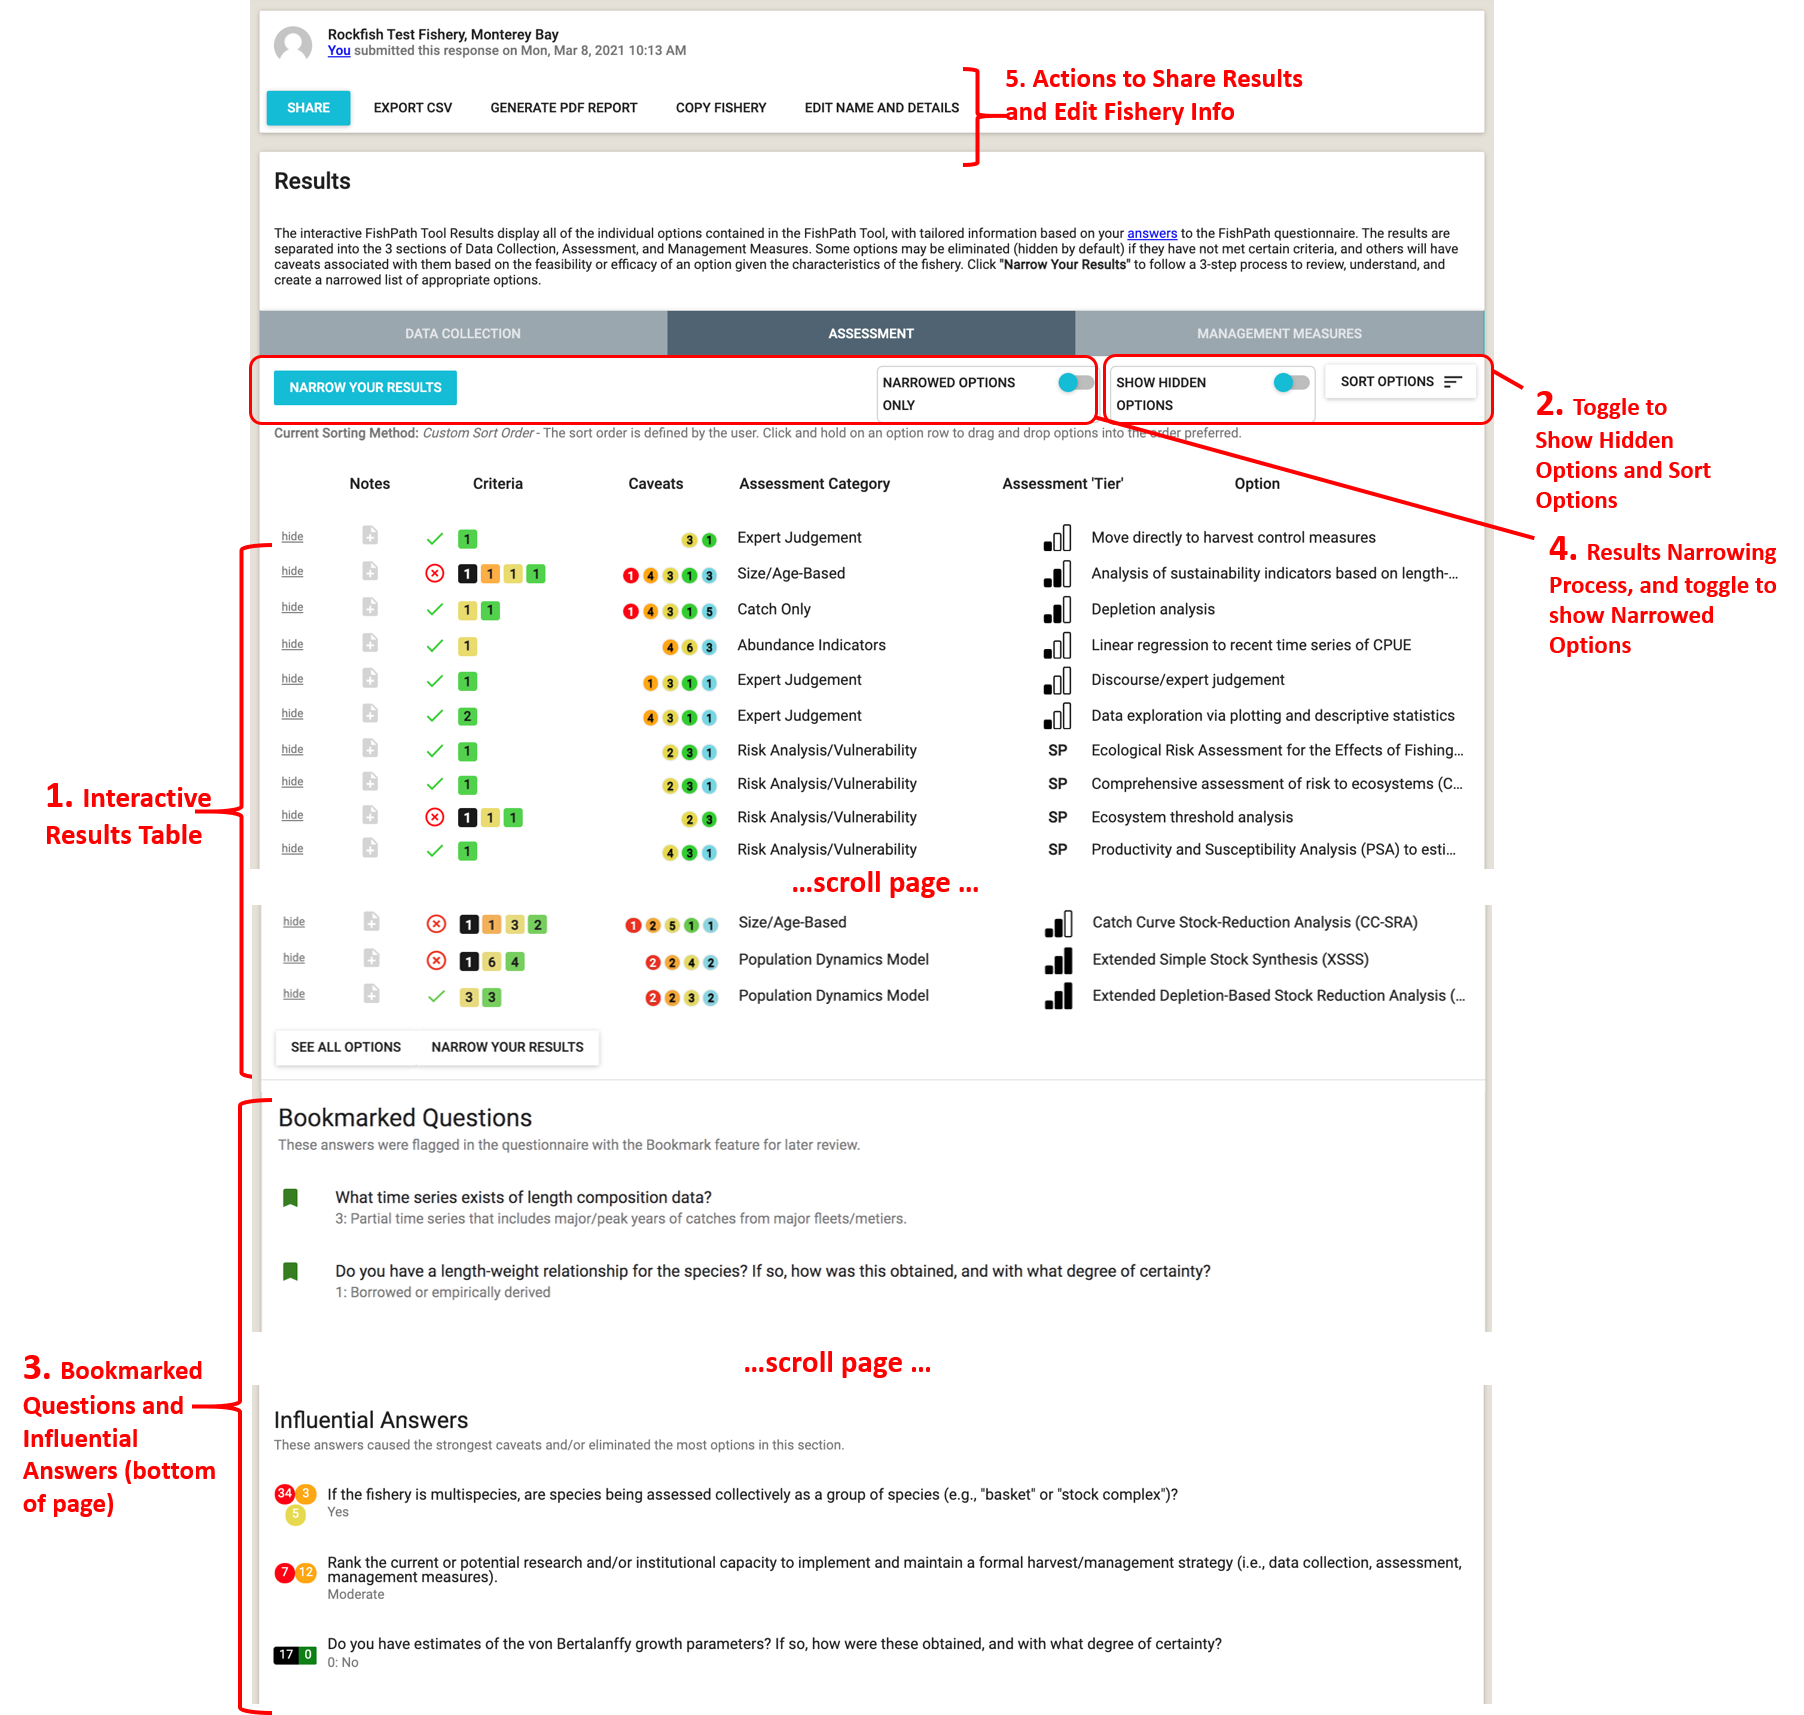
\includegraphics[width=0.95\linewidth]{images/results-components} 

}

\caption{Key components (red labels 1-5) of the FishPath Interactive Tool Results Page.}\label{fig:results-components}
\end{figure}

\hypertarget{Results-Actions}{%
\section{Actions to Share Results and Edit Fishery Info}\label{Results-Actions}}

At the top of the Results Page, the user may either ``Share'', ``Export CSV'', ``Generate PDF Report'', ``Copy'', or ``Edit Name and Details'' for their fishery (Figure \ref{fig:results-components}).

\begin{itemize}
\tightlist
\item
  \textbf{Share:} This will generate a link that allows the user to share a fishery with someone. The user simply needs to send the link and the recipient will have view-only access to this fishery from their active account. A shared fishery can be saved under someone else's FishPath account, and they can make a copy of it to separately edit, if needed. Tip: when creating a copy of a shared fishery in a user account, it is useful to rename the fishery so that edits are tracked under this new name.
\item
  \textbf{Export CSV:} This allows users to export the question and answer list from the saved questionnaire, as well as a simple results file, as a .csv file.
\item
  \textbf{Generate PDF Report:} Allows the user to create a .PDF of the FishPath results, with all notes captured. The PDF report provides detailed information on each option and their associated caveats and criteria related to the fishery. Users can select to see a report for the ``full list'' of options, or for a specified list of ``top options''.
\item
  \textbf{Copy Fishery:} This allows users to make a copy of a fishery's results, be these their own, or from a shared link. To rename that fishery and edit it under a different name, the user should select the ``Edit Name and Details'' button.
\item
  \textbf{Edit Name and Details:} This allows users to edit the information entered on the Fishery Information form (name, species, geography, etc.)
\end{itemize}

\hypertarget{interactive-results-table}{%
\section{Interactive Results Table}\label{interactive-results-table}}

The results table lists all the available options for the section of interest in rows. Each row summarizes the criteria met and failed, and the caveats invoked (see also ``Criteria and Caveat Questions'' section above). Each option can be selected and expanded to view its description and results in more detail. A guide to the content contained in each row is listed below.

\hypertarget{table-structure}{%
\subsection{Table Structure}\label{table-structure}}

Figure \ref{fig:single-row} displays a single row from an example results table. The single row represents one option in the FishPath tool, and the details of this singe row are as follows:

\begin{figure}

{\centering 
\includegraphics[width=0.95\linewidth]{images/single-row} 

}

\caption{Headings of the FishPath tool results table.}\label{fig:single-row}
\end{figure}

\begin{itemize}
\tightlist
\item
  \textbf{Hide/Unhide:} Any option for which one or more of its minimum criteria have not been met by the fishery is automatically ``hidden'' (greyed-out) by the FishPath tool. For any option, including those not meeting minimum criteria, users may manually click this link to ``hide'' the option, or click ``hidden'' or reinstate it.
\end{itemize}

\begin{center}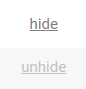
\includegraphics[width=0.1\linewidth]{images/hide} \end{center}

\begin{itemize}
\tightlist
\item
  \textbf{Notes:} As within the questionnaire, notes may be written and saved (with a secure internet connection) for each option. For example, notes may be taken on fishery-specific details (not covered within the questionnaire) on why that option may or may not be a good fit, or to record the user's or user groups overall evaluation of the option, given its associated criteria and caveats. Alternatively, notes may be taken if options are hidden or reinstated, to justify that choice as documentation. Notes are be included in the PDF report.
\end{itemize}

\begin{center}
\includegraphics[width=0.15\linewidth]{images/notes} \end{center}

\begin{itemize}
\tightlist
\item
  \textbf{Criteria (Data Collection and Assessment sections):} The criteria column provides information on whether the fishery meets the minimum conditions required to undertake the option. As explained above, the Management Measures section does not include criteria. If the fishery has met all of the minimum criteria required for the option, a green check is displayed. On the other hand, if a fishery has not met one or more of the minimum criteria required for the option, a red X is displayed (and the option is automatically ``hidden''). The numbered boxes next to the red ``X'' indicate the number of criteria met (green) and unmet (black). For the assessment section only, criteria also have associated ``traffic light'' colored (black, red, orange, yellow, green) guidance to encourage FishPath users to explicitly consider the possible uncertainty associated with the quality of their fishery's information (with black equating to a minimum criterion not having been met). The numbers within in each symbol, are the subset of the total criteria for that option that were not met (black), and that invoked (red, orange, yellow) uncertainty warnings, and positive attributes (green), as triggered by questionnaire responses.
\end{itemize}

\begin{center}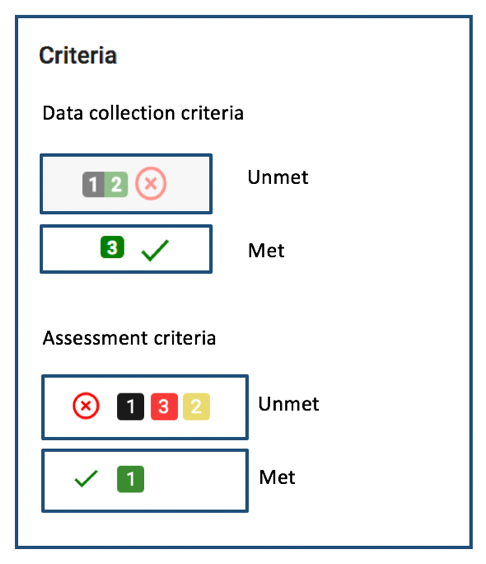
\includegraphics[width=0.35\linewidth]{images/criteria} \end{center}

\begin{itemize}
\item
  \textbf{Caveats:} The format of the caveats column is identical across all three sections. Caveats are shown as colored circles with numbers indicating the total number of questionnaire responses that invoked a caveat of that particular color. There are three types of caveats:

  \begin{enumerate}
  \def\labelenumi{\arabic{enumi}.}
  \tightlist
  \item
    \textbf{Cautionary, or warning caveats:} these are marked as red, orange, and yellow circles with the severity or strength of the caveat corresponding to the color (red being highest). These give cautionary guidance based on an attribute of a fishery. For example, if the user responded that the species of interest is susceptible to barotrauma, this would invoke a red caveat against size limits as a management measure, since the fishing-induced mortality of the released (under- or over-sized) fish would render size limits ineffective.
  \item
    \textbf{Positive attributes:} A green colored caveat provides reasoning for why the option might be well-suited for the fishery on the basis on a of a user response in the questionnaire.
  \item
    \textbf{Static caveats:} Turquoise colored caveats are static caveats that need to be considered for an option, regardless of the fishery or the questionnaire responses. A static caveat is independent of specific fishery circumstances and as such are always present. These include key assessment assumptions, for example, that the assessment option assumes that fishery selectivity has not changed over time, or that the assessment method cannot explicitly address uncertainty.
  \end{enumerate}
\end{itemize}

\begin{center}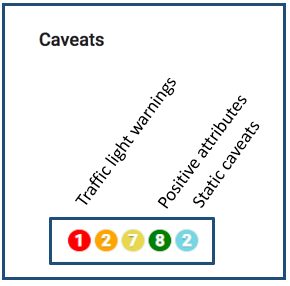
\includegraphics[width=0.35\linewidth]{images/caveats} \end{center}

\begin{itemize}
\item
  \textbf{(Data) Category:} The Category column allows the user to view the options by categories. This column is different for each section. In the Data Collection Section, this column is titled ``Data Category'', showing the four categories of the type of data that may be collected (see also ``Data Collection Section Results'' above). In the Assessment Section, this column is titled either ``Input-Based Category'' or ``Output-Based Category'', reflecting two sorting options available for organizing the assessment option results. In the Management Measures Section, this column is simply titled ``Category'' and displays the categories of management measures.
\item
  \textbf{Option:} This is the name of the option being considered.
\end{itemize}

\hypertarget{full-option-details}{%
\subsection{Full Option Details}\label{full-option-details}}

Each row in the Results Table displays the option name with summarized results for each option. When users click on any option, a pop-up box appears, which provides full details of the option itself, together with the detail of the criteria and caveats invoked.

First, a description of the option is provided, together with relevant references, and contact information (if available or appropriate). For the Data Collection options, the types of data that may be collected using the option are summarized. For the Assessment section, where available, links to assessment packages are provided.

Next, the invoked criteria and caveats are summarized by (Figure \ref{fig:opt-desc})

\begin{itemize}
\tightlist
\item
  Criteria not met,
\item
  Met criteria,
\item
  Cautionary caveats,
\item
  Positive attribute caveats, and
\item
  Static caveats
\end{itemize}

Next to each, there are individual drop-down menus where the user can find the specific detail on each individual criterion and caveat, along with the question and response that invoked the criterion or caveat.

\begin{figure}

{\centering 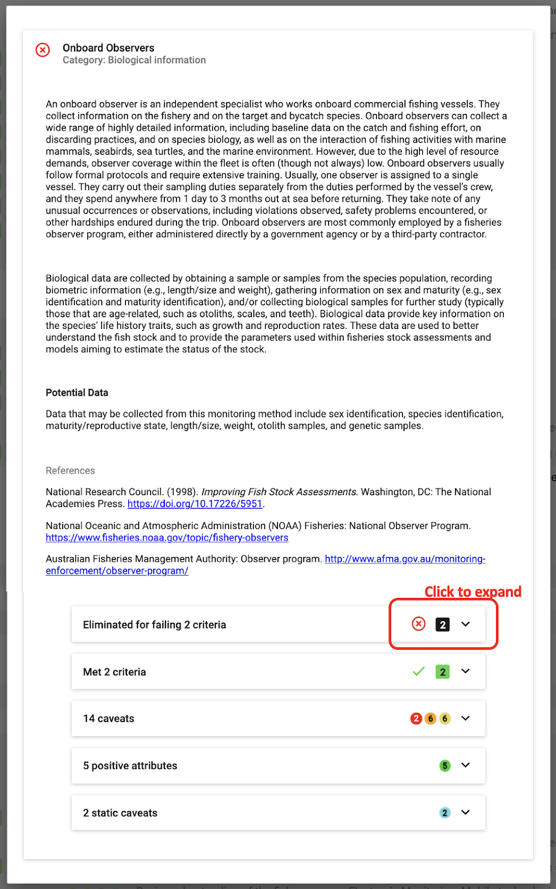
\includegraphics[width=0.5\linewidth]{images/option-description} 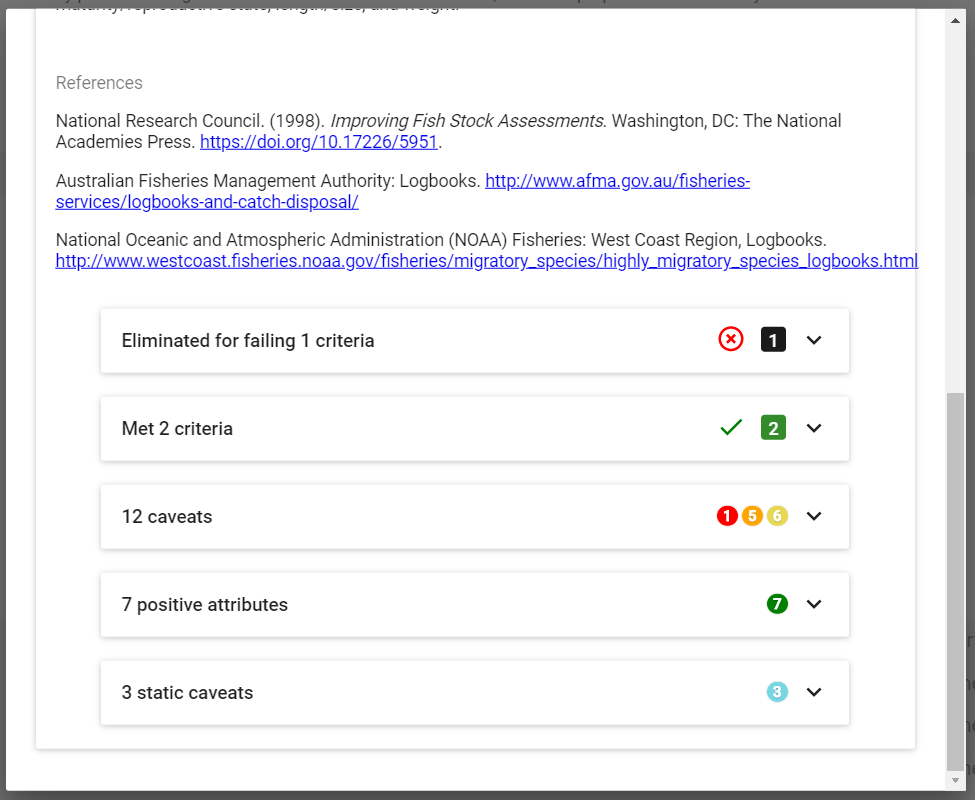
\includegraphics[width=0.5\linewidth]{images/option-result-details} 

}

\caption{Example of pop-up box that appears when clicking on each option.}\label{fig:opt-desc}
\end{figure}

\textbf{Criteria drop-down box (Figures \ref{fig:crit-drop-down}-\ref{fig:assessment-crit-drop-down})}: Each criterion drop-down shows the relevant question with the user's response shown (highlighted in black) relative to the minimum required level for that option (where green coloring starts on left) (Figure \ref{fig:crit-drop-down}). The Assessment section assigns traffic light colors to levels above the minimum, indicating their relative uncertainty and thus the relative caution that should be taken (Figure \ref{fig:assessment-crit-drop-down}).

\begin{figure}

{\centering 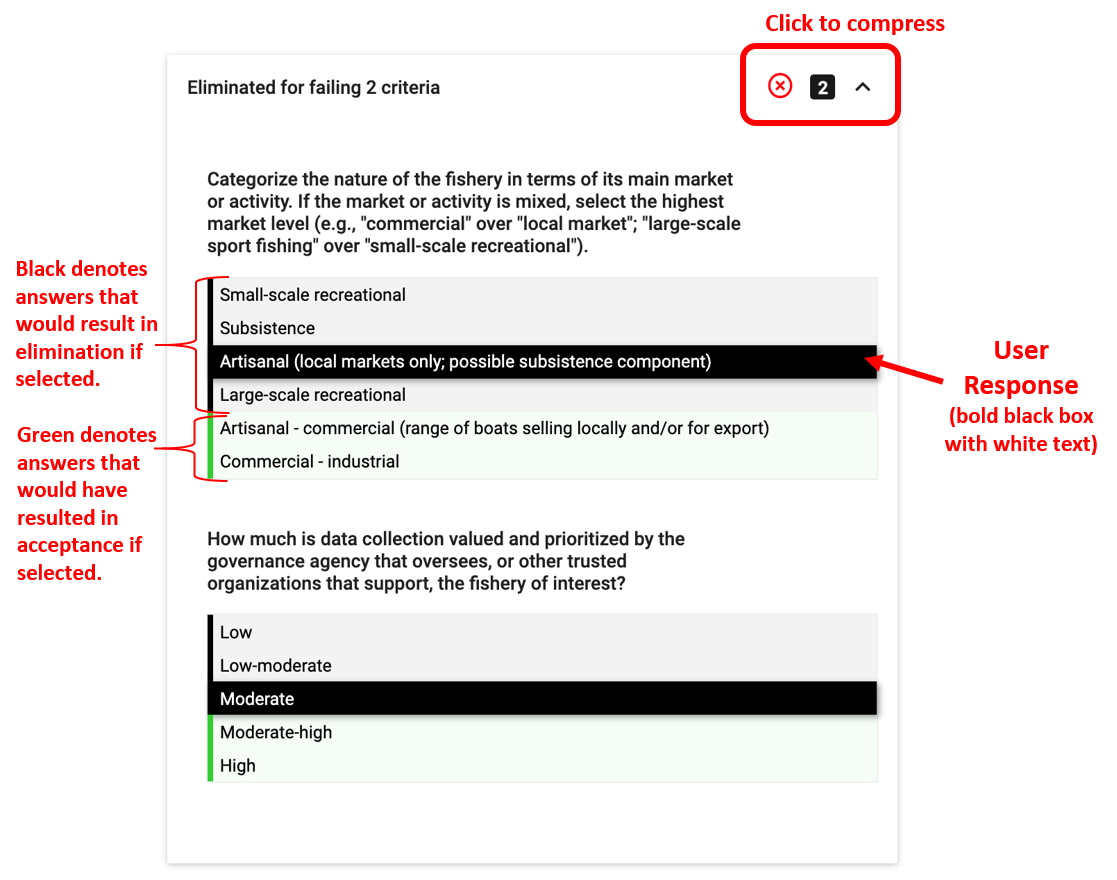
\includegraphics[width=0.75\linewidth]{images/crit-drop-down} 

}

\caption{Example drop-down menu with details for an option in the Data Collection section that was eliminated for failing two criteria. The bold, black box and white text indicates the user answer to the question. The black answer options indicate those that result in elimination if selected. The green answer options indicate those that would have resulted in acceptance if selected.}\label{fig:crit-drop-down}
\end{figure}

\begin{figure}

{\centering 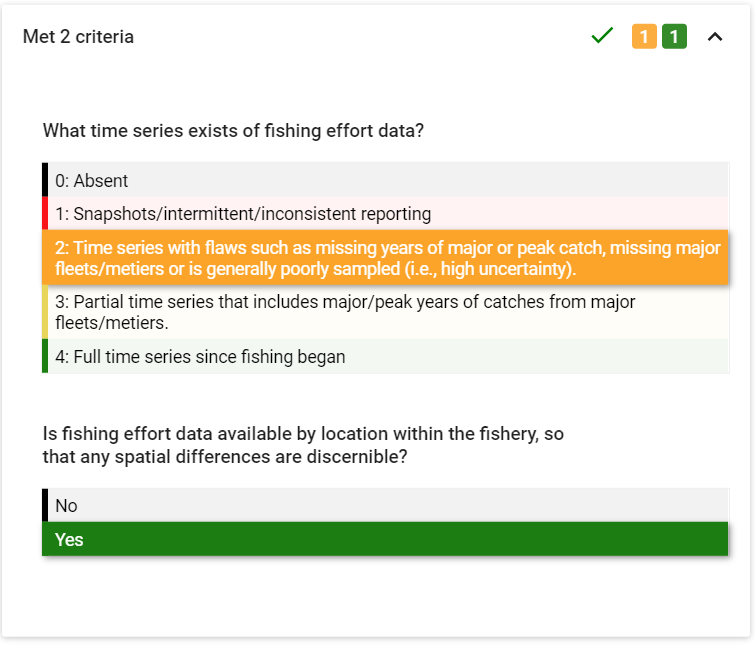
\includegraphics[width=0.75\linewidth]{images/assessment-crit-drop-down} 

}

\caption{Example drop-down menu with details for an option in the Assessment section that has passed criteria, but indicating the user to take caution regarding the uncertainty in the fishing effort data. Red indicates high uncertainty in the data. Green indicates low uncertainty.}\label{fig:assessment-crit-drop-down}
\end{figure}

\textbf{Caveat Drop-Down Box (Figures \ref{fig:cav-drop-down}-\ref{fig:static-cav-drop-down})}: Each individual caveat box displays the FishPath question with the user's answer in grey text, followed by caveat text related to the use of the option in the fishery in the context of that particular question response. The color of each box reflects the caveat color (see caveat descriptions above): cautionary caveats shaded yellow, orange or red; positive attributes shaded green; and static caveats shaded in turquoise.

\begin{figure}

{\centering 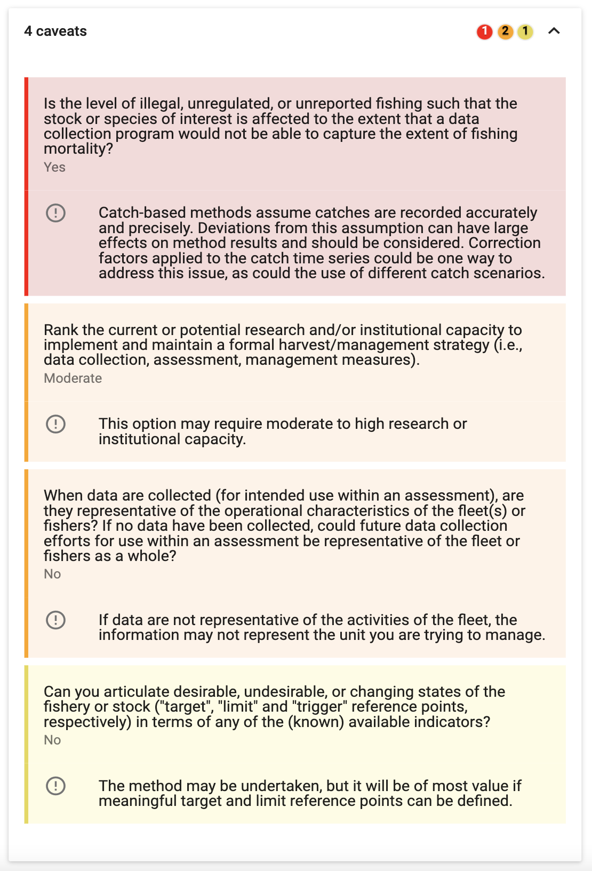
\includegraphics[width=0.75\linewidth]{images/cav-drop-down} 

}

\caption{Example caveat drop-down menu with details for an option for which questionnaire responses invoked 8 cautionary caveats (2 orange, 6 yellow, as shown at the top right corner of the drop-down menu).}\label{fig:cav-drop-down}
\end{figure}

\begin{figure}

{\centering 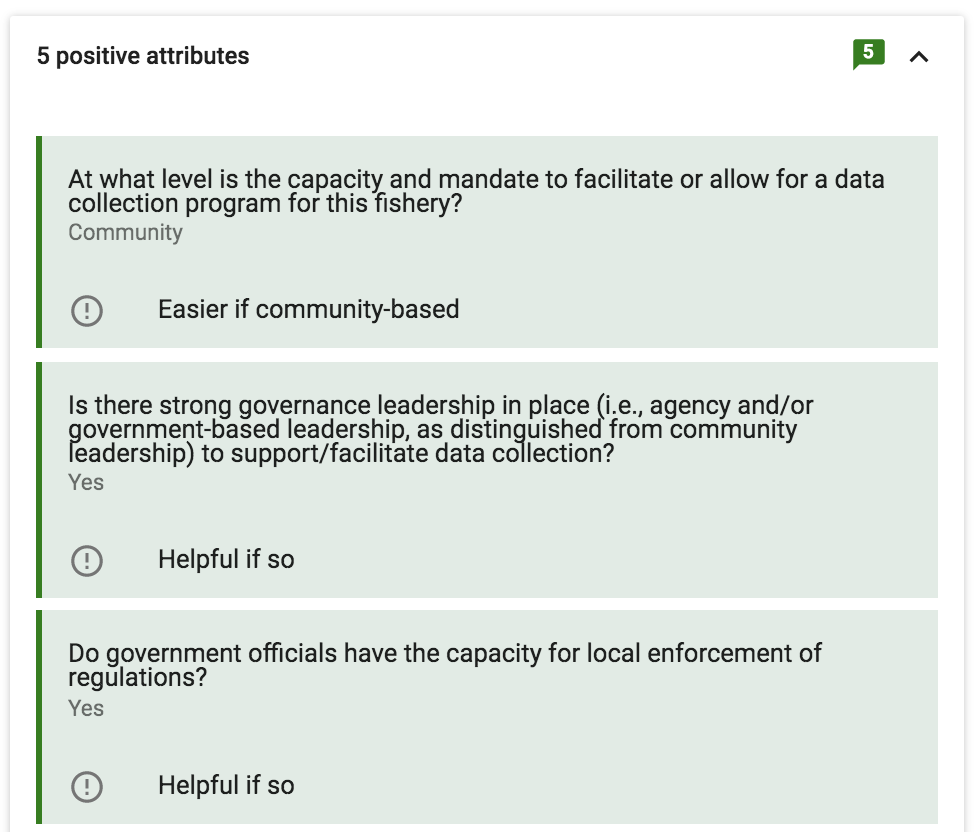
\includegraphics[width=0.75\linewidth]{images/pos-attr-drop-down} 

}

\caption{Example drop-down menu of positive attributes for an option for which questionnaire responses invoked 5 positive attributes (shown at the top right corner of the drop-down menu).}\label{fig:pos-attr-drop-down}
\end{figure}

\begin{figure}

{\centering 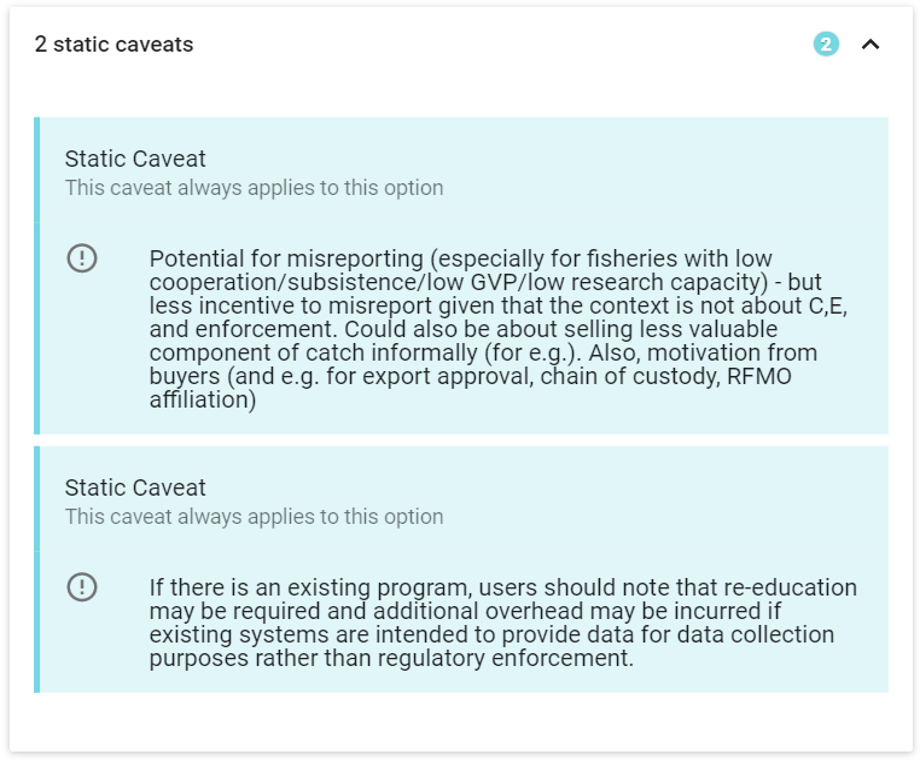
\includegraphics[width=0.75\linewidth]{images/static-cav-drop-down} 

}

\caption{Example static caveat drop-down menu for an option with 3 static caveats (shown at the top right corner of the drop-down menu). Each individual static caveat box displays grey text to note “This caveat always applies to this option”, and a short explanation of the static caveat.}\label{fig:static-cav-drop-down}
\end{figure}

\hypertarget{more-information-on-options-within-the-3-results-sections}{%
\subsection{More Information on Options within the 3 Results Sections}\label{more-information-on-options-within-the-3-results-sections}}

\hypertarget{data-collection-section-results}{%
\subsubsection{Data Collection Section Results}\label{data-collection-section-results}}

The Data Collection section of the FishPath tool includes a range of data collection options (from market surveys, to logbooks and observer programs). These data collection options are subdivided according to the broad category of data that may be collected, as these influence the viability of the data collection option. The four data categories in the FishPath tool are: 1) biological information; 2) data that yield a basic understanding of the fishery; 3) data that can inform temporal trend analyses (data time series), and 4) data that are of a sufficient quality to inform a model-based stock assessment.

\hypertarget{assessment-section-results}{%
\subsubsection{Assessment Section Results}\label{assessment-section-results}}

The Assessment section of the FishPath tool allows the user to understand which data-limited stock assessment methods are available and best suited to their fishery. In the FishPath tool, an assessment is defined as any analysis or performance indicator that gives useful information for management by direct or indirect measures of stock status. This could range from a ``cause for concern'' arising from expert judgement, qualitative risk assessments, values of empirical indicators relative to pre-defined trigger levels, multiple indicator frameworks, to life history analyses that provide estimates of fishing mortality, F, or fishing mortality at maximum sustainable yield FMSY, catch-only models, size or length based approaches, to population dynamics model-fitting approaches that estimate biomass.

\hypertarget{management-measure-section-results}{%
\subsubsection{Management Measure Section Results}\label{management-measure-section-results}}

A management measure is the form of control used to manage the fishing mortality. Once the desired management measures have been identified (for example, size limits, or catch adjustments in response to quantitative assessment outcomes), they are adjusted via ``decision rules'', or ``harvest control rules''. These specify the strength and nature of the pre-agreed management action to be taken given the status of the fishery, as determined by the assessment. Management measures can take many forms including spatial, temporal, effort, catch, and gear related restrictions. The FishPath tool does not have any minimum criteria listed for management measures, but instead uses cautionary caveats. Multiple management measures can and should be used together. The FishPath tool results do not prescribe or give guidance on the specific form of the harvest rule, nor the strength of adjustment in response to assessment outcomes. However, the FishPath tool does direct users to resources and tools that can support in this process, located within the description of each option.

\hypertarget{show-hidden-options-and-sort-options}{%
\section{Show Hidden Options and Sort Options}\label{show-hidden-options-and-sort-options}}

The ``Show Hidden Options'' Toggle (Figure \ref{fig:show-hidden-sort}) allows users to display or not display those options that have been ``hidden'' (greyed out) in the results table. When shown, ``hidden'' options will appear in grey.

\begin{figure}

{\centering 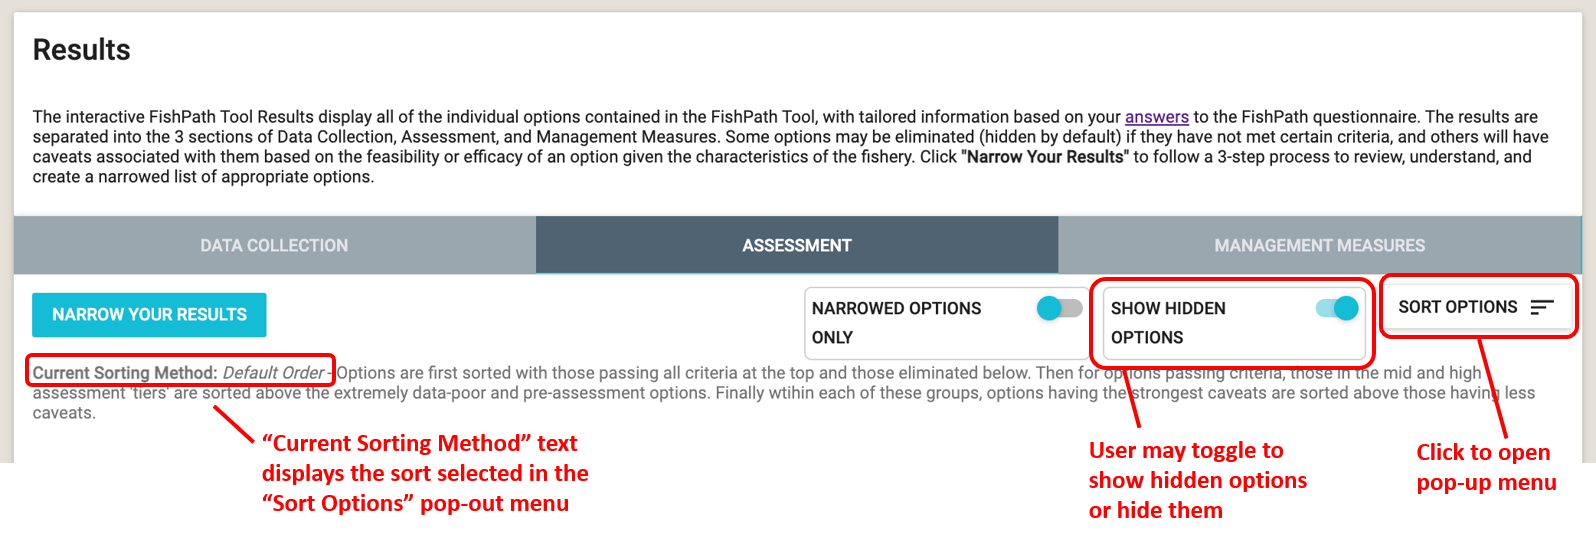
\includegraphics[width=0.75\linewidth]{images/show-hidden-options-and-sort} 

}

\caption{Results page with the “Show Hidden Options” Toggle and “Sort Options” in a red circle.}\label{fig:show-hidden-sort}
\end{figure}

The ``Sort Options'' functionality allows the user to arrange and view the options in different ways. This does not affect the results or shortlisting of options; it is merely a means to organize and display the results.

After clicking ``Sort Options'', a pop-up box (Figure \ref{fig:filter-and-sorting}) appears with the ability to sort the options by:

\begin{itemize}
\tightlist
\item
  In the Assessment section only, there is an additional option to sort by two categories: ``Output-Based Category'' (i.e., according to the general type of output generated by the assessment method or option); or ``Input-Based Category'' (i.e., according to the main form of input required by the assessment or option).
\item
  \textbf{Default Order:} The default sort is to list all options that did not meet minimum criteria at the bottom (automatically greyed out as hidden options), with the options for which the highest number of cautionary caveats were invoked at the top for review.
\item
  \textbf{Customized Sort Order:} This maintains the current sort order but allows users to return to the results table and ``drag and drop'' options into the preferred order.
\item
  \textbf{Sort by option name:} Sorts options alphabetically by option name.
\item
  \textbf{Sort by category:} Sorts options alphabetically by category name. For the Assessment section, users first select the Category Display that they want to display and sort by.
\end{itemize}

Clicking a Sort option automatically sorts the options on the screen. After making selections on the Sort window, users can click outside of the pop-up onto the results table to return to the results.
The current sort selected is shown at the top of the results table at ``Current Sorting Method'' (Figure \ref{fig:show-hidden-sort}).

\begin{figure}

{\centering 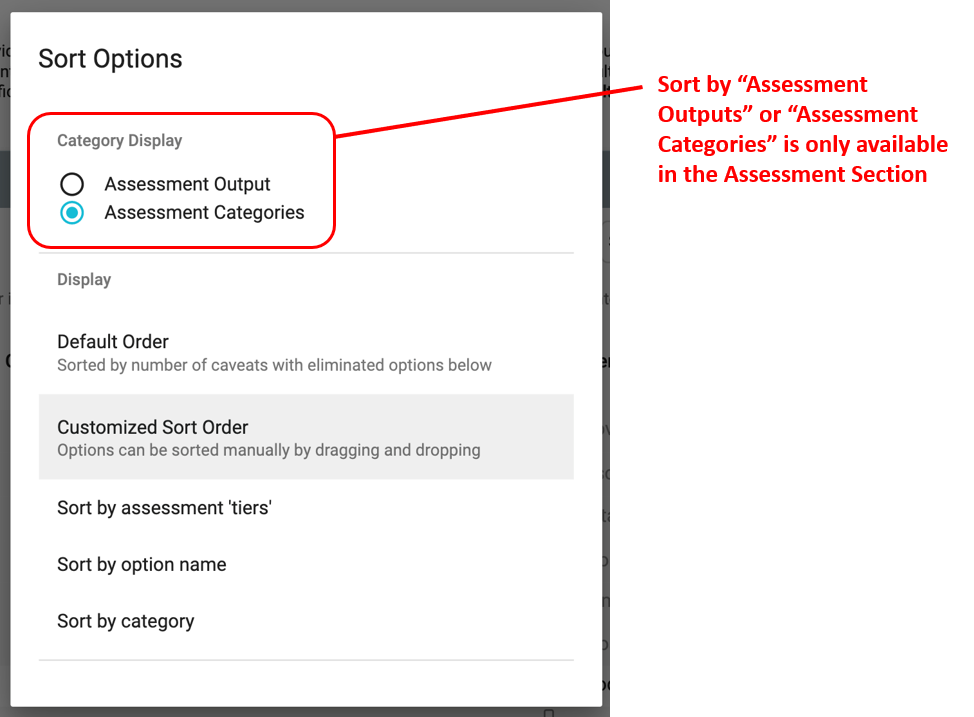
\includegraphics[width=0.5\linewidth]{images/filter-and-sorting-assessment} 

}

\caption{Sort Options pop-up box.}\label{fig:filter-and-sorting}
\end{figure}

\hypertarget{bookmarked-questions-and-influential-answers}{%
\section{Bookmarked Questions and Influential Answers}\label{bookmarked-questions-and-influential-answers}}

If the user scrolls to the bottom of the results screen (below results table), they are provided with a summary list of the questions bookmarked by the user, together with a list of ``Influential Answers'', and, finally, a ``See All Answers'' link.

\hypertarget{bookmarked-questions}{%
\subsection{Bookmarked Questions}\label{bookmarked-questions}}

All questions that were ``bookmarked'' during the questionnaire will be listed here (Figure \ref{fig:flagged-questions}). Users can select each question to get a detailed list of all caveats invoked or criteria not met based on the response. Users can also select each question to change the answer, add notes, or remove bookmark. It is highly recommended to review these questions and invoked caveats so that users can update their response or provide more detailed notes on the response, based on seeing how the response impacts results.

\begin{figure}

{\centering 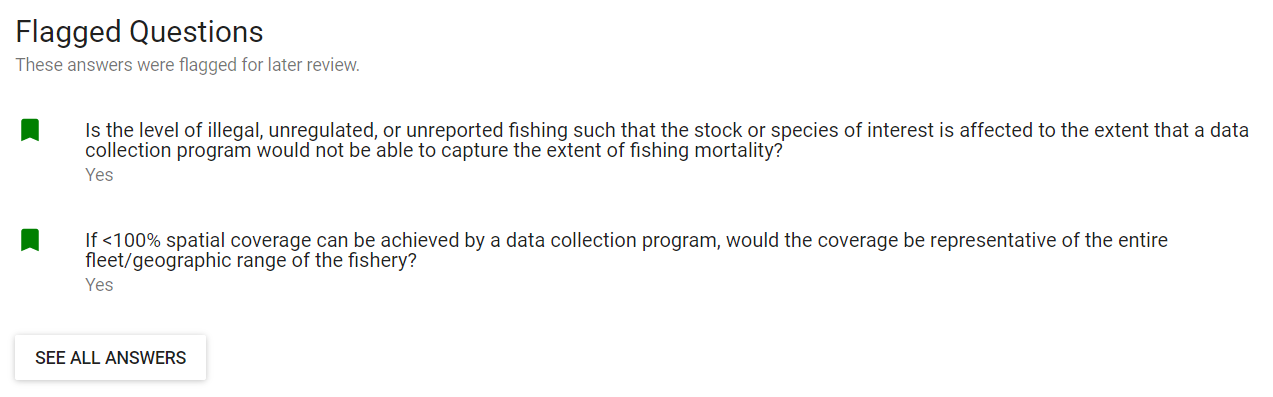
\includegraphics[width=0.95\linewidth]{images/flagged-questions} 

}

\caption{List of bookmarked questions.}\label{fig:flagged-questions}
\end{figure}

\hypertarget{influential-answers}{%
\subsection{Influential Answers}\label{influential-answers}}

The ``Influential Answers'' list is a summary of the questions and user responses that invoked the most eliminating criteria (by number), together with the number of caveats and criteria invoked, by assigned traffic light color (Figure \ref{fig:influential-answers}). The caveats invoked by the question are displayed (color strength and number) to its left.

It is recommended to review this list prior to entering the results narrowing process (described below), to better understand some of the key challenges facing the fishery. Users can select any question on this list to change an answer, add notes to the question, and see a list of all impacted options and their associated caveats (Figure \ref{fig:influential-answers-expanded}).

\begin{figure}

{\centering 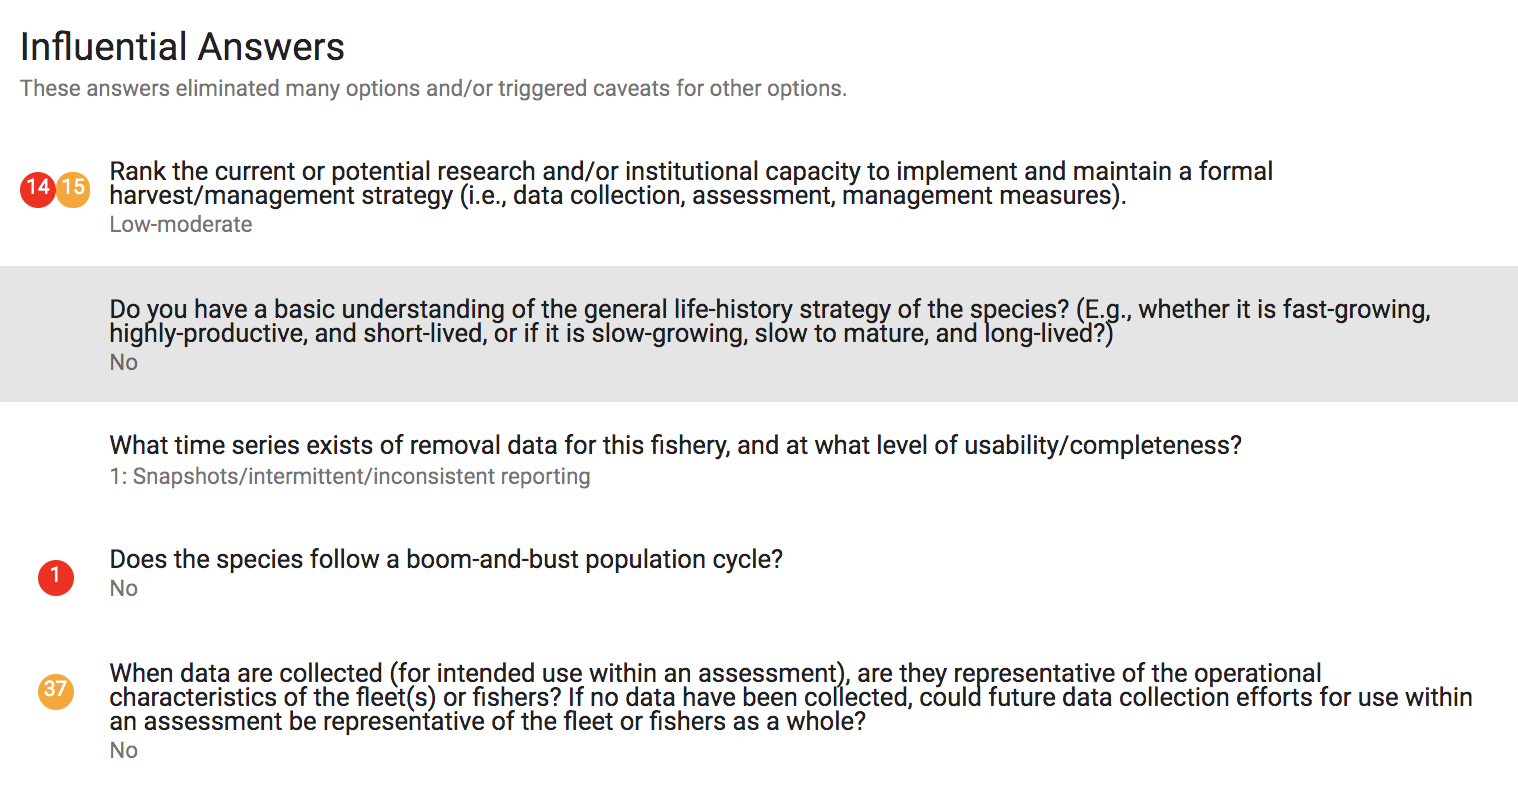
\includegraphics[width=0.95\linewidth]{images/influential-answers} 

}

\caption{List of influential answers.}\label{fig:influential-answers}
\end{figure}

\begin{figure}

{\centering 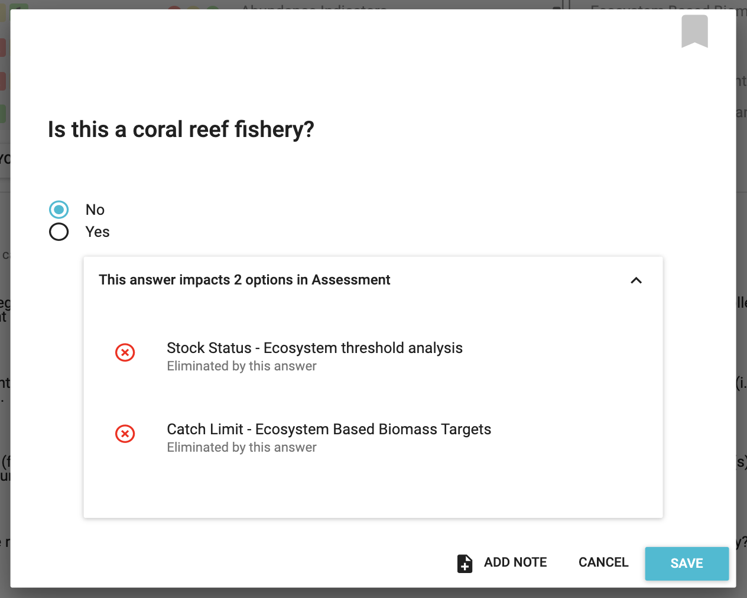
\includegraphics[width=0.75\linewidth]{images/influential-answers-expanded} 

}

\caption{Impacted options for a question.}\label{fig:influential-answers-expanded}
\end{figure}

At the bottom of these lists, there is a link to ``See All Answers'' (as well as at the top of the results screen under ``Answers''). These links take users to a full list of answers from each section, showing all information, including the number of caveats invoked, and any bookmarked questions. This is a good resource for users wanting to review the questionnaire responses for a fishery. Answers may also be changed and notes added, which update after clicking ``Save''.

\hypertarget{Results-Narrowing}{%
\section{Results Narrowing Process}\label{Results-Narrowing}}

Typically, the FishPath questionnaire process results in a long list of potential options that are presented to the user. The challenge is to then refine this to a workable shortlist of options that can be reviewed in further detail, and around which a draft harvest strategy can be developed. This can be a daunting task, given the number of options, and the large amount of detail around the criteria and caveats invoked against each. As such, the Results Review provides guidance as to how to undertake the task of narrowing the list of viable harvest strategy components.

The Results Narrowing process prompts the user through a series of steps to further refine and narrow the options for their fishery, and to consider detail about the application of each option in the fishery. The goal is to finish with a short list of defensible, appropriate and documented options for the fishery.

First, the user accesses the Results Narrowing process by selecting the ``Review Top Options'' button located above the Results Table in the Results Screen. (See Figure \ref{fig:results-overview})

After clicking on ``Review Top Options'', the user is directed to a step-wise results review process (Figure \ref{fig:results-review}). Each step of the results review process contains an ``Instructions'' box with clear steps, as well as the ability to access different steps of the results review process through ``Back'', ``Exit Review'' and ``Next Step'' (Figure \ref{fig:results-review}). Across the top of the page, the user views steps in the process:

\begin{figure}

{\centering 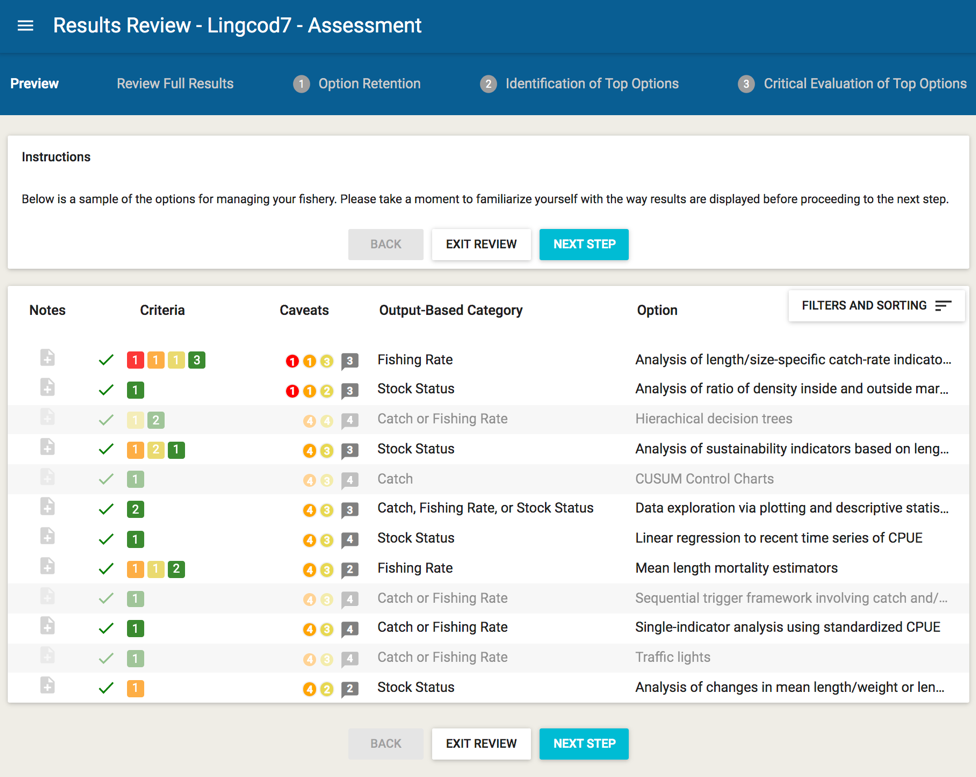
\includegraphics[width=0.95\linewidth]{images/results-review} 

}

\caption{Overview of the FishPath Tool results screen and results review process.}\label{fig:results-review}
\end{figure}

The narrowing process (done as a group exercise or by independent users), consists of the following major steps:

\begin{enumerate}
\def\labelenumi{\arabic{enumi}.}
\tightlist
\item
  \textbf{Option Retention (Figure \ref{fig:review-step-1}):} The goal of the first step is to hide all options that are clearly not viable for the fishery due to failure to meet minimum criteria, logistical, political, or other major reasons. Users should carefully review the list to hide these options, as well as un-hide options that they want to reinstate. Specific instructions are included on the screen in this step of the process, including questions to consider as narrowing the list.
\end{enumerate}

\begin{figure}

{\centering 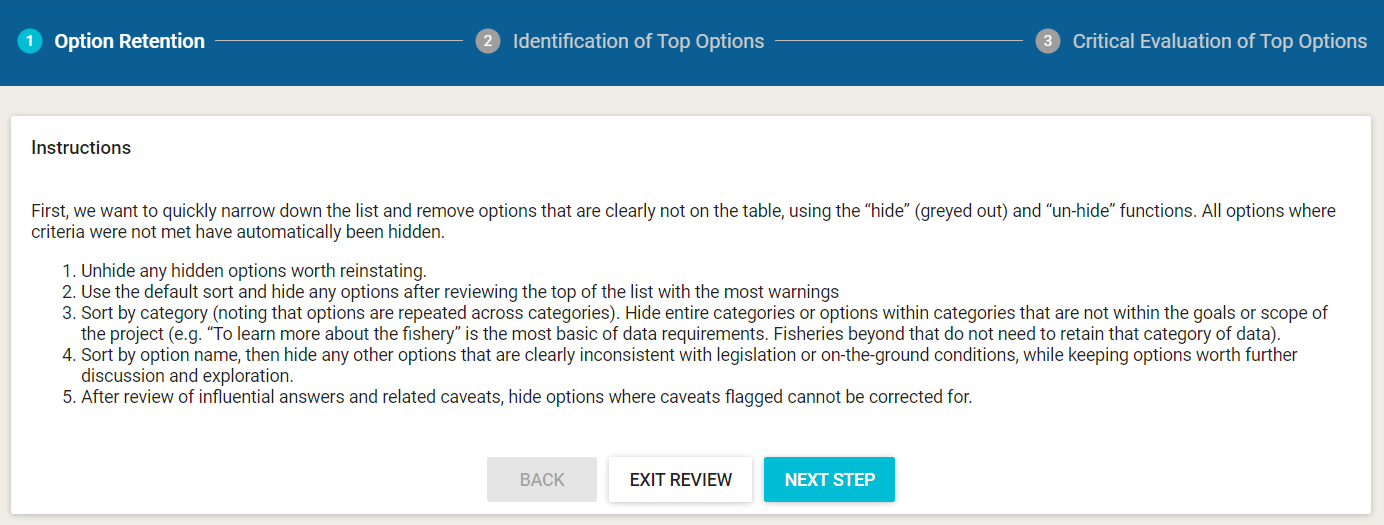
\includegraphics[width=0.95\linewidth]{images/review-step-1} 

}

\caption{Step 1, Option Retention, in the results review process.}\label{fig:review-step-1}
\end{figure}

\begin{enumerate}
\def\labelenumi{\arabic{enumi}.}
\setcounter{enumi}{1}
\tightlist
\item
  \textbf{Identification of Top Options (Figure \ref{fig:review-step-2}):} In this step, users review each remaining option to identify a short list of starred options that will be seriously considered and explored in more detail. Users should familiarize themselves with the sorting feature and the influential answer list (see above) to facilitate this process. When comparing options, users should compare the number of cautionary caveats and criteria, their relative strength, and the ratio of cautionary caveats to positive attribute caveats. Specific instructions are included on the screen in this step of the process.
\end{enumerate}

\begin{figure}

{\centering 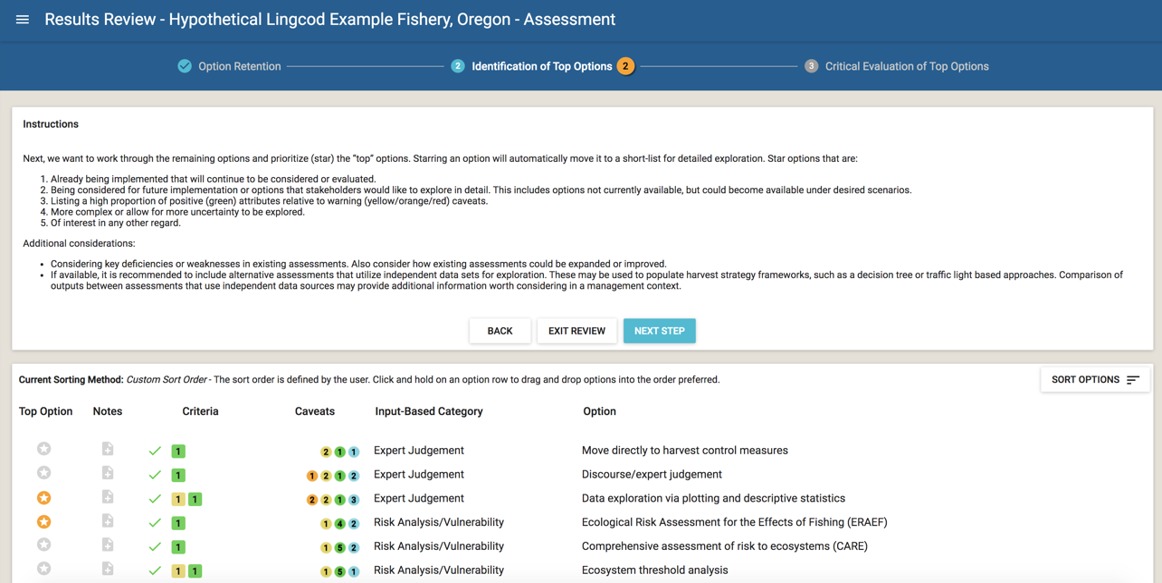
\includegraphics[width=0.95\linewidth]{images/review-step-2} 

}

\caption{Step 2, Identification of Top Options, in the results review process.}\label{fig:review-step-2}
\end{figure}

\begin{enumerate}
\def\labelenumi{\arabic{enumi}.}
\setcounter{enumi}{2}
\tightlist
\item
  \textbf{Critical Evaluation of Top Options (Figure \ref{fig:review-step-3}):} In the final step, users can more critically evaluate the top options by considering each criterion and caveat in complete detail, and, potentially, ranking the options in order of potential. To facilitate this process, users can export a report that lists the top options and all of their details.
\end{enumerate}

\begin{figure}

{\centering 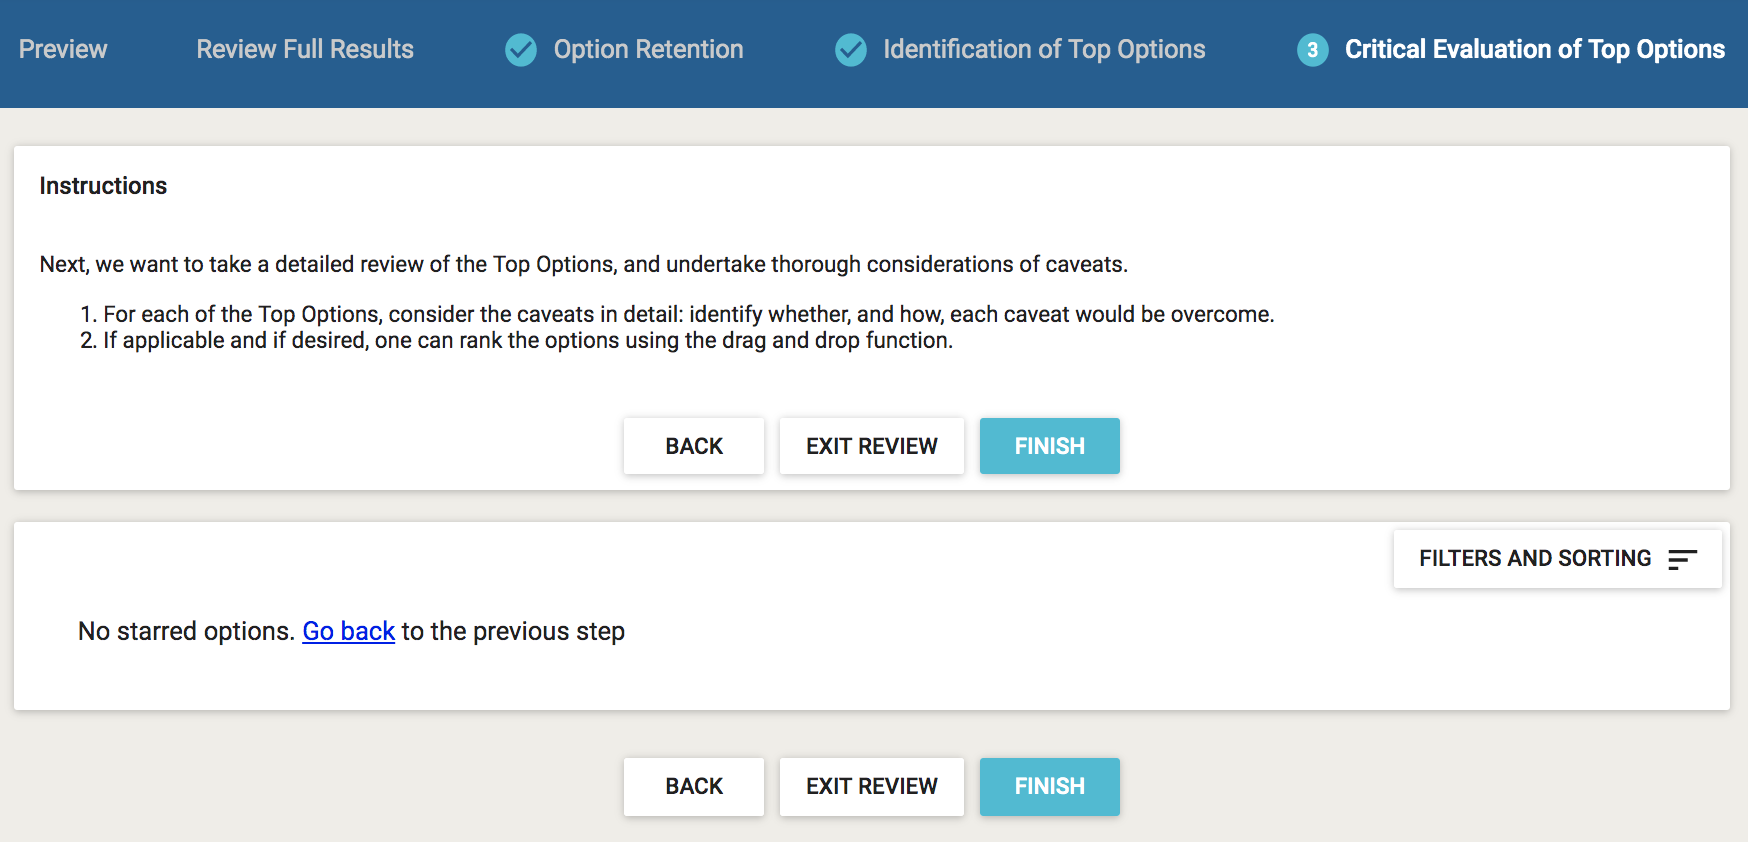
\includegraphics[width=0.95\linewidth]{images/review-step-3} 

}

\caption{Step 3, Critical Evaluation of Top Options, in the results review process.}\label{fig:review-step-3}
\end{figure}

\hypertarget{appendix-appendix}{%
\appendix}


\hypertarget{fishpath-tool-frequently-asked-questions}{%
\chapter{FishPath Tool Frequently Asked Questions}\label{fishpath-tool-frequently-asked-questions}}

\textbf{How do I submit feedback about content or user experience?}

FishPath benefits from the expertise and feedback of the global community of FishPath tool users. Users are encouraged to submit feedback about the FishPath tool, ultimately helping to improve the tool. There are three ways to submit feedback:

\begin{enumerate}
\def\labelenumi{\arabic{enumi}.}
\tightlist
\item
  Submit issue on GitHub\\
\item
  The ``Help us improve the FishPath tool'' button on FishPath Tool Dashboard. The user is prompted to categorize their feedback as ``Content Related'' or ``Software Issue''.
\item
  Email \href{mailto:support@fishpath.org}{\nolinkurl{support@fishpath.org}}
\end{enumerate}

\textbf{How is my feedback addressed and incorporated?}

The FishPath Tool undergoes periodic updates to ensure that the tool reflects the latest fisheries science and management information. User-submitted feedback and suggestions, as well as information from periodic reviews of the tool, are collated and synthesized by the FishPath Core Team and addressed and incorporated.

\textbf{How often is the FishPath tool updated?}

Every 6 months.

\textbf{How will I know about updates to the FishPath tool?}

All FishPath users will receive an email every 6 months when updates are published. Common changes that users may expect are the addition of new options and questions. When they revisit the FishPath tool, they may need to answer new questions to see results and they may have new options in the results.

\textbf{Are answers to new questions also updated in ``copied fisheries''?}

Once a fishery is copied, changes in the original or copied fishery will have no effect on the other.

\hypertarget{terms}{%
\chapter{FishPath Tool Terms of Service}\label{terms}}

\textbf{Last revised on October 23, 2018}

The Nature Conservancy (``TNC,'' ``we,'' ``us,'' or ``our'') are pleased to provide FishPath and related software, data, websites, instructions, and services (``FishPath'') to you. If you are using FishPath on behalf of a business (such as your employer), that business accepts these terms of service (``Terms'') by your use. In that case, the words ``You'' and ``Your'' in these Terms refer to both you and that business.

The Terms govern Your access to and use of FishPath, so please carefully read them and Our Privacy Policy before using FishPath. By registering on the FishPath websites and using FishPath, You agree to be bound by these Terms and by our Privacy Policy. If You don't agree with these Terms and our Privacy Policy, You cannot use FishPath or FishPath data in any way or at any time.

\hypertarget{fishpath-data-your-rights-and-your-privacy}{%
\subsubsection*{FishPath Data: Your Rights and Your Privacy}\label{fishpath-data-your-rights-and-your-privacy}}
\addcontentsline{toc}{subsubsection}{FishPath Data: Your Rights and Your Privacy}

We developed FishPath as a user-friendly application to help users diagnose the challenges in their fishery and select appropriate options for data collection, stock assessment, and management measures. FishPath allows You to use Your fishery information (Your ``Submission''). Your Submission to FishPath is voluntary. If You submit information to FishPath, these Terms do grant us the right to see and use Your Submission to improve the functionality of the tool as appropriate. We may copy and share an anonymized aggregation of information from submissions, potentially including Your Submission, with the public. However, we will not share Your submission nor Your information in any non aggregated format.

Please refer to our \href{https://www.nature.org/en-us/about-us/who-we-are/accountability/privacy-policy/}{Privacy Policy} for a description of how we collect, use and disclose FishPath information, including Your Submission. We have the right to withdraw or change FishPath. As we describe below, we will not be liable to You if for any reason all or any part of FishPath is unavailable at any time or for any length of time.

\hypertarget{your-responsibilities}{%
\subsubsection*{Your Responsibilities}\label{your-responsibilities}}
\addcontentsline{toc}{subsubsection}{Your Responsibilities}

Only make a Submission if You have all necessary rights to share the information with us, including but not limited to use with FishPath. You are solely responsible for your conduct and Your Submission while using FishPath. It is Your responsibility to ensure that You have the rights or permission needed to comply with these Terms.

Respect the law. Do not use FishPath for any fraudulent or unlawful purpose including violations of statutory, regulatory or contractual law. Respect copyright, privacy, trade secret, data protection, fish \& wildlife and all other laws. Do not attempt to impersonate any other individual on FishPath; if You identify yourself, You must always use Your true identity.

Without our express written consent, You may not use, display, mirror, or frame FishPath, any element within FishPath, or any proprietary elements belonging to us (including but not limited to our logos and marks). In addition to adhering to all applicable laws and regulations, You may NOT do any of the following:

\begin{itemize}
\tightlist
\item
  resell FishPath or data from FishPath, or any portion thereof;
\item
  access or search the FishPath data by using any engine, software, tool, agent, device or mechanism (including spiders, robots, crawlers, data mining tools or the like) other than the software and/or search agents that We provide or authorize;
\item
  probe, scan, tamper with, or test the vulnerability of FishPath or any of our systems or networks;
\item
  avoid, breach, deactivate, impair, or circumvent any security or authentication measures, including those that protect FishPath and its data;
\item
  attempt to decipher, decompile, disassemble or reverse engineer any of the software used to provide FishPath;
\item
  interfere with, or attempt to interfere with, the access of any user, host or network, including, without limitation, by sending a virus, overloading, or flooding FishPath;
\item
  encourage or enable anyone else to do any of the foregoing.
\end{itemize}

We have the right to investigate violations of these Terms or conduct that affect FishPath or our systems or networks. We may also consult and cooperate with law enforcement authorities to prosecute users who violate the law.

\hypertarget{rights-you-grant-in-your-information}{%
\subsubsection*{Rights You Grant in Your Information}\label{rights-you-grant-in-your-information}}
\addcontentsline{toc}{subsubsection}{Rights You Grant in Your Information}

By making Your Submission, You grant us a non-exclusive, transferable, sublicensable, worldwide, perpetual, royalty-free license to use, copy, modify, create derivative works based upon, distribute, publicly display, publicly perform and distribute Your Submission. We will not, however, share or distribute specific notes You submit for Your fishery.

\hypertarget{rights-that-we-grant-you}{%
\subsubsection*{Rights That We Grant You}\label{rights-that-we-grant-you}}
\addcontentsline{toc}{subsubsection}{Rights That We Grant You}

Subject to Your compliance with these Terms, we grant You a limited, non-exclusive, non-transferable, non-sublicensable, worldwide, royalty-free license to use the FishPath software, instructions, and websites and to view, copy, display, and create derivative works from the FishPath output that we make available from the FishPath site for Your management of Your fishery.

You may not: (i) copy, modify or create derivative works based on the FishPath software; (ii) distribute, transfer, sublicense, lease, or rent the FishPath software to any third party; or (iii) reverse engineer, decompile or disassemble the FishPath software.

Using FishPath or uploading Data does not give You ownership of any intellectual property rights in FishPath (other than your own Submission). We and our licensors exclusively own all right, title and interest in and to FishPath, including all associated intellectual property rights. You acknowledge that copyright, trademark, and other laws of the United States and foreign countries protect FishPath. You agree not to remove, alter or obscure any copyright, trademark, service mark or other proprietary rights notices incorporated in or accompanying FishPath.

These Terms do not grant You the right to use any of our branding or logos or names. You must not use our names or logos or branding without our written permission.

\hypertarget{modifying-our-terms-of-service}{%
\subsubsection*{Modifying our Terms of Service}\label{modifying-our-terms-of-service}}
\addcontentsline{toc}{subsubsection}{Modifying our Terms of Service}

We may update these Terms from time to time, in our sole discretion. We may notify You of such updates by any reasonable means, such as by posting the revised Terms on the FishPath website. Please look at the ``LAST UPDATED'' legend above to see when these Terms were last revised. Your use of FishPath after the posting of any revised Terms means that You accept and agree to be bound by the revised Terms. If You don't agree to be bound by the revised Terms, then You may not use FishPath anymore. You can stop using FishPath at any time. We may also stop providing FishPath or add or create new limits to FishPath at any time.

\hypertarget{disclaimers-limited-liability-and-indemnity}{%
\subsubsection*{Disclaimers, Limited Liability and Indemnity}\label{disclaimers-limited-liability-and-indemnity}}
\addcontentsline{toc}{subsubsection}{Disclaimers, Limited Liability and Indemnity}

As we describe in more detail below, FishPath and its data are a general information resource and are provided solely ``AS IS'' and ``AS AVAILABLE'' without warranty of any kind. You should not construe publication of FishPath data as a warranty or guarantee of the quality or availability of any goods or services or technical support.

\hypertarget{disclaimers-and-limitation-of-liability}{%
\subsubsection*{DISCLAIMERS AND LIMITATION OF LIABILITY}\label{disclaimers-and-limitation-of-liability}}
\addcontentsline{toc}{subsubsection}{DISCLAIMERS AND LIMITATION OF LIABILITY}

ALL CONTENT ON FISHPATH IS PROVIDED ``AS IS'' AND ``AS AVAILABLE'' WITHOUT WARRANTY OF ANY KIND, EITHER EXPRESS OR IMPLIED. WITHOUT LIMITING THE FOREGOING, WE EXPLICITLY DISCLAIM ANY AND ALL WARRANTIES OF MERCHANTABILITY, FITNESS FOR A PARTICULAR PURPOSE, QUIET ENJOYMENT, OR NON-INFRINGEMENT, AND ANY AND ALL WARRANTIES ARISING OUT OF COURSE OF DEALING OR USAGE OF TRADE. TNC MAKES NO WARRANTY AS TO THE QUALITY, ACCURACY, COMPLETENESS, TIMELINESS, OR RELIABILITY OF FISHPATH OR ANY FISHPATH CONTENT. YOUR USE OF FISHPATH IS AT YOUR SOLE RISK.

TNC MAKES NO REPRESENTATIONS OR WARRANTIES THAT YOUR USE OF FISHPATH WILL MEET YOUR NEEDS OR BE UNINTERRUPTED, SECURE, OR ERROR FREE. USERS ARE RESPONSIBLE FOR TAKING ALL NECESSARY PRECAUTIONS TO ENSURE THAT ANY CONTENT YOU MAY OBTAIN FROM THE SERVICES IS FREE OF VIRUSES OR OTHER HARMFUL CODE.

TO THE MAXIMUM EXTENT PERMITTED BY LAW, WE SHALL NOT BE LIABLE FOR CREATING, PRODUCING, MAINTAINING, OPERATING, OR PROVIDING FISHPATH OR FISHPATH CONTENT, UNDER ANY THEORY BASED IN CONTRACT, WARRANTY, TORT (INCLUDING NEGLIGENCE), PRODUCT LIABILITY, STRICT LIABILITY, OR OTHER LEGAL THEORY. THIS LIMITATION ON LIABILITY INCLUDES ANY AND ALL INDIRECT, INCIDENTAL, SPECIAL, EXEMPLARY OR CONSEQUENTIAL DAMAGES, INCLUDING LOST PROFITS, LOSS OF DATA OR GOODWILL, SERVICE INTERRUPTION, COMPUTER DAMAGE OR SYSTEM FAILURE OR THE COST OF SUBSTITUTE SERVICES ARISING OUT OF OR IN CONNECTION WITH THESE TERMS OR FROM THE USE OF OR INABILITY TO USE FISHPATH, EVEN IF WE HAVE BEEN ADVISED OF THE POSSIBILITY OF SUCH DAMAGES.

THE ABOVE EXCLUSIONS AND LIMITATIONS OF DAMAGES ARE FUNDAMENTAL ELEMENTS OF THE BASIS OF THE BARGAIN BETWEEN YOU AND US.

\hypertarget{indemnity}{%
\subsubsection*{Indemnity}\label{indemnity}}
\addcontentsline{toc}{subsubsection}{Indemnity}

You agree to release, indemnify, defend and hold harmless TNC, our subsidiaries and affiliates, and our and their respective officers, directors, agents, partners and employees, from and against any claims, disputes, demands, liabilities, damages, losses, and costs and expenses, including, without limitation, reasonable legal and accounting fees arising out of or in any way connected with (i) Your access to or use of FishPath, (ii) Your Submission, or (iii) Your violation of these Terms.

\hypertarget{termination}{%
\subsubsection*{Termination}\label{termination}}
\addcontentsline{toc}{subsubsection}{Termination}

We may terminate Your access to and use of FishPath, at our sole discretion, at any time and without notice to You. Upon any termination, discontinuation or cancellation of FishPath, all provisions of these Terms that by their nature should survive will survive. This includes, for example ownership provisions, warranty disclaimers, and limitations of liability.

\hypertarget{general-terms}{%
\subsubsection*{General Terms}\label{general-terms}}
\addcontentsline{toc}{subsubsection}{General Terms}

These Terms are the entire and exclusive agreement between You and us regarding FishPath, and they supersede any prior agreements between You and us regarding FishPath.

These terms do not create any third party beneficiary rights. You may not assign or transfer these Terms, by operation of law or otherwise, without our prior written consent. Subject to the foregoing, these Terms will bind your successors and permitted assigns. We may freely assign or transfer these Terms without restriction.

If You do not comply with these Terms, and we do not take action right away, this does not mean that we are giving up any rights that we may have to take action in the future or seek all available remedies.

If it turns out that a particular provision of these Terms is not fully valid or enforceable, that provision will be enforced to the maximum extent permissible, and this will not affect any other Terms.

All claims arising out of this Agreement or relating to FishPath will be governed by the laws of the State of California, excluding the application of its conflicts of law rules. Any legal action or proceeding arising out of this Agreement or relating to these Services shall be brought exclusively in a state or federal court in or for San Francisco, California. You agree that any and all disputes, claims and causes of action arising out of, or connected with these Terms or Your Submission shall be resolved individually, without resort to any form of class action.

  \bibliography{book.bib,packages.bib}

\end{document}
